% =====================================================================
%  NVIDIA GPU Architectures after Volta  --  a lecture on the compute
%  GPUs from Turing (2018) to Vera Rubin (2026) and the announced road
%  beyond: what each generation added to the SM, the tensor cores and
%  their number formats, the memory system (HBM2 to HBM4), NVLink and
%  NVSwitch up to the rack-scale NVL72 and NVL144, the Grace and Vera
%  CPUs, the systems built from them, and the software that drives it.
%  Same visual language as "Introduction to GPU Architectures".
%
%  Compile:  pdflatex nvidia_after_volta_tutorial.tex   (run twice)
%  Self-contained: every figure is TikZ/pgfplots source in this file.
%
%  Conventions
%   * \stage{n} before a frame sets the accent color and highlights the
%     matching chip in the footer strip.
%   * Numbers quoted from a paper or a vendor report name the source;
%     numbers labeled "derived" were computed from quoted ones; curves
%     labeled "illustrative" are sketches, not data; $^\dagger$ marks
%     vendor documentation, model cards, blogs and commentary.
% =====================================================================
\documentclass[aspectratio=169,11pt]{beamer}

% ---------- fonts ----------------------------------------------------
\usepackage[scaled=0.92]{helvet}        % Helvetica-like sans for text
\renewcommand{\ttdefault}{cmtt}         % Computer Modern mono for tokens
\usefonttheme[onlymath]{serif}          % classic serif math
\usepackage{amsmath,amssymb,bm}
\usepackage{booktabs,array}
\usepackage{graphicx}


% ---------- graphics -------------------------------------------------
\usepackage{tikz}
\usepackage{pgfplots}
\pgfplotsset{compat=1.17}
\usetikzlibrary{arrows.meta,positioning,calc,fit,backgrounds,
                decorations.pathreplacing,shapes.geometric}

% ---------- palette --------------------------------------------------
\definecolor{ink}{HTML}{1F2937}     % text, residual stream
\definecolor{muted}{HTML}{6B7280}   % secondary text
\definecolor{hair}{HTML}{D9DDE4}    % hairlines
\definecolor{paper}{HTML}{FCFCFA}   % slide background
\definecolor{tok}{HTML}{5F6F85}     % tokens / tokenizer
\definecolor{emb}{HTML}{0CA678}     % embeddings
\definecolor{posc}{HTML}{7048E8}     % positional information
\definecolor{attn}{HTML}{E8590C}    % attention
\definecolor{mlp}{HTML}{1C7ED6}     % MLP / feed-forward
\definecolor{norm}{HTML}{5C940D}    % normalization
\definecolor{outc}{HTML}{D6336C}     % unembedding / softmax / sampling
\definecolor{trn}{HTML}{9C6644}     % training and scaling
\colorlet{qc}{attn}                 % queries
\definecolor{kc}{HTML}{F59F00}      % keys
\definecolor{vc}{HTML}{1098AD}      % values
\colorlet{kct}{kc!70!black}         % key color, darkened for text
\colorlet{stagec}{ink}              % accent of the current stage

% ---------- beamer look ----------------------------------------------
\setbeamertemplate{navigation symbols}{}
\setbeamercolor{background canvas}{bg=paper}
\setbeamercolor{normal text}{fg=ink}
\setbeamercolor{frametitle}{fg=ink}
\setbeamersize{text margin left=8mm,text margin right=8mm}
\setbeamertemplate{itemize item}{\raisebox{0.25ex}{\tiny\color{stagec}$\blacksquare$}}
\setlength{\leftmargini}{1.1em}
\hyphenpenalty=10000 \exhyphenpenalty=10000   % no hyphenation on slides

% stage = which part of the pipeline the slide belongs to
\newcount\stageno \stageno=1
\newcommand{\stage}[1]{\global\stageno=#1\relax
  \ifcase#1\or\colorlet{stagec}{ink}\or\colorlet{stagec}{tok}%
  \or\colorlet{stagec}{emb}\or\colorlet{stagec}{attn}%
  \or\colorlet{stagec}{mlp}\or\colorlet{stagec}{posc}%
  \or\colorlet{stagec}{trn}\or\colorlet{stagec}{outc}%
  \or\colorlet{stagec}{vc}\or\colorlet{stagec}{ink}\fi}

\makeatletter
% title: accent bar + title + one-line claim (the frame subtitle)
\setbeamertemplate{frametitle}{%
  \nointerlineskip\vspace*{3.6mm}%
  \begin{tikzpicture}[x=1mm,y=1mm]
    \useasboundingbox (0,0) rectangle (144,10.5);
    \fill[stagec,rounded corners=0.5mm] (0,0.3) rectangle (1.5,10.2);
    \ifx\insertframesubtitle\@empty
      \node[anchor=west,inner sep=0,text=ink,
            font=\fontsize{15}{17}\selectfont\bfseries] at (4.2,5.2) {\insertframetitle};
    \else
      \node[anchor=west,inner sep=0,text=ink,
            font=\fontsize{15}{17}\selectfont\bfseries] at (4.2,7.1) {\insertframetitle};
      \node[anchor=west,inner sep=0,text=muted,
            font=\fontsize{8.6}{10}\selectfont] at (4.2,2.0) {\insertframesubtitle};
    \fi
  \end{tikzpicture}}
\makeatother

% footer: pipeline strip with the current stage lit, plus page number
\setbeamertemplate{footline}{%
  
\begin{tikzpicture}[x=1mm,y=1mm]
    \useasboundingbox (0,0) rectangle (160,7.2);
    \coordinate (c0) at (7.2,4.0);
    \foreach \lab/\col [count=\i,remember=\i as \prev (initially 0)] in
      {Overview/ink,Turing/tok,Ampere/emb,Hopper/attn,Ada/mlp,
       Blackwell/posc,Rubin/trn,Systems/outc,Software/vc,Wrap-up/ink}{
      \ifnum\i=\stageno
        \node[anchor=west,inner xsep=1.5mm,inner ysep=0.75mm,rounded corners=0.7mm,
              fill=\col,text=white,text height=1.5ex,text depth=0.35ex,
              font=\fontsize{5.8}{7}\selectfont\bfseries] (c\i) at ([xshift=0.8mm]c\prev.east) {\lab};
      \else
        \node[anchor=west,inner xsep=1.5mm,inner ysep=0.75mm,
              text=muted!80,text height=1.5ex,text depth=0.35ex,
              font=\fontsize{5.8}{7}\selectfont] (c\i) at ([xshift=0.8mm]c\prev.east) {\lab};
      \fi}
    \node[anchor=east,inner sep=0,text=muted,
          font=\fontsize{6.5}{8}\selectfont] at (152,4.0)
          {\insertframenumber\,/\,\inserttotalframenumber};
  \end{tikzpicture}}

% ---------- TikZ vocabulary ------------------------------------------
\tikzset{
  >={Stealth[length=4.6pt,width=4pt]},
  flow/.style={->,line width=0.8pt,draw=ink!70},
  thinflow/.style={->,line width=0.5pt,draw=ink!55},
  % component box (tinted) and its solid variant; argument = color
  comp/.style={rounded corners=2.2pt,draw=#1,fill=#1!12,line width=0.8pt,
               align=center,inner sep=4pt,font=\small,text=ink},
  fillbox/.style={rounded corners=2.2pt,fill=#1,text=white,align=center,
                inner sep=4pt,font=\small\bfseries},
  % a token
  chip/.style={rounded corners=1.8pt,fill=tok!14,draw=tok!55,line width=0.5pt,
               font=\ttfamily\footnotesize,inner xsep=3.5pt,inner ysep=2.5pt,
               text height=1.5ex,text depth=0.45ex,text=ink},
  cchip/.style={chip,fill=#1!16,draw=#1!75},
  lab/.style={font=\scriptsize,text=muted,inner sep=1.5pt},
  txt/.style={font=\footnotesize,text=ink,align=flush left,inner sep=0pt},
  plus/.style={circle,draw=ink,fill=paper,line width=0.75pt,inner sep=0pt,
               minimum size=9.5pt,font=\scriptsize\bfseries},
  brace/.style={decorate,decoration={brace,amplitude=3.5pt},draw=muted,line width=0.6pt},
}

% \cells{x}{y}{size}{color}{shade,shade,...}: a row of vector cells
\newcommand{\cells}[5]{%
  \foreach \sh [count=\ci from 0] in {#5}{%
    \fill[#4!\sh!white,draw=paper,line width=0.4pt]
      ({#1+\ci*#3},{#2}) rectangle ++(#3,#3);}}

% \rgrid{x}{y}{rows}{cols}{size}{color}{seed}: a matrix with varied shading
\newcommand{\rgrid}[7]{%
  \foreach \ri in {1,...,#3}{\foreach \ci in {1,...,#4}{%
    \pgfmathtruncatemacro\sh{16+mod(\ri*37+\ci*53+\ri*\ci*11+#7*29,8)*10}%
    \fill[#6!\sh!white,draw=paper,line width=0.4pt]
      ({#1+(\ci-1)*#5},{#2+(#3-\ri)*#5}) rectangle ++(#5,#5);}}}

% \barh{x}{y}{length}{color}: one horizontal bar of a bar chart
\newcommand{\barh}[4]{\fill[#4,rounded corners=0.8pt] ({#1},{#2-0.13}) rectangle ++({#3},0.26);}

% \valgrid{x}{y}{size}{color}{scale}{mask}{\rows}: matrix shaded by value.
% (x,y) is the top-left corner; \rows is a macro holding {a,b,..},{..},..
% With mask=1 the cells above the diagonal are drawn as blocked.
\newcommand{\valgrid}[7]{%
  \edef\vglist{#7}%
  \foreach \row [count=\r from 0] in \vglist {\foreach \v [count=\c from 0] in \row {%
    \pgfmathtruncatemacro\sh{min(100,\v*#5)}%
    \pgfmathtruncatemacro\msk{and(#6>0,\c>\r)}%
    \ifnum\msk=1
      \fill[tok!10,draw=paper,line width=0.4pt] ({#1+\c*#3},{#2-(\r+1)*#3}) rectangle ++(#3,#3);
    \else
      \fill[#4!\sh!white,draw=paper,line width=0.4pt] ({#1+\c*#3},{#2-(\r+1)*#3}) rectangle ++(#3,#3);
    \fi}}}

% the running attention example: Alice thanked Bob because she
\def\Sraw{{2.0,0.7,1.3,0.4,1.1},{1.8,1.2,0.9,1.6,0.5},{0.6,1.5,1.9,0.8,1.4},
          {0.8,1.6,0.9,1.1,2.1},{3.1,0.9,1.4,1.0,1.5}}          % scores
\def\Aw{{1.00,0,0,0,0},{.65,.35,0,0,0},{.14,.35,.51,0,0},
        {.18,.39,.19,.24,0},{.62,.07,.11,.08,.12}}              % softmax rows

% paper figure: \paperfig{file}{width}{Figure n}
\newcommand{\paperfig}[3]{%
  \begin{tikzpicture}
    \node[inner sep=0] (img) {\includegraphics[width=#2]{#1}};
    \node[anchor=north east,font=\fontsize{5.5}{6}\selectfont,text=muted,
          rounded corners=1pt,fill=ink!6,inner sep=2pt] at ([xshift=-1mm,yshift=-1mm]img.north east) {report, #3};
  \end{tikzpicture}}
% background panel: \bgpanel{x}{y}{width}{title}{body}  (anchor north west)
\newcommand{\bgpanel}[5]{%
  \node[anchor=north west,inner sep=0] at (#1,#2) {%
    \begin{tikzpicture}
      \node[anchor=north west,text width=#3,align=flush left,font=\footnotesize,text=ink,
            inner xsep=8pt,inner ysep=6pt,rounded corners=3pt,fill=stagec!7] (bp)
            {{\color{stagec}\bfseries\scriptsize #4}\\[3pt]#5};
      \fill[stagec,rounded corners=1.5pt] (bp.north west) rectangle ([xshift=3pt]bp.south west);
    \end{tikzpicture}};}
% same panel with a smaller body font, for denser slides
\newcommand{\bgpanels}[5]{%
  \node[anchor=north west,inner sep=0] at (#1,#2) {%
    \begin{tikzpicture}
      \node[anchor=north west,text width=#3,align=flush left,font=\scriptsize,text=ink,
            inner xsep=8pt,inner ysep=6pt,rounded corners=3pt,fill=stagec!7] (bp)
            {{\color{stagec}\bfseries\scriptsize #4}\\[3pt]#5};
      \fill[stagec,rounded corners=1.5pt] (bp.north west) rectangle ([xshift=3pt]bp.south west);
    \end{tikzpicture}};}
% stat tile: \stat{x}{y}{value}{label}{color}
\newcommand{\stat}[5]{%
  \node[anchor=north west,inner sep=0] at (#1,#2) {%
    \begin{tikzpicture}
      \node[anchor=north west,minimum width=3.2cm,minimum height=1.45cm,rounded corners=3pt,
            fill=#5!10,draw=#5!50,line width=0.6pt] (t) {};
      \node[anchor=north west,font=\fontsize{15}{16}\selectfont\bfseries,text=#5!85!black,inner sep=0]
            at ([xshift=7pt,yshift=-7pt]t.north west) {#3};
      \node[anchor=south west,font=\scriptsize,text=ink,inner sep=0,text width=2.9cm,align=left]
            at ([xshift=7pt,yshift=6pt]t.south west) {#4};
    \end{tikzpicture}};}

% small source tag inside a figure: \srctag{x}{y}{text}
\newcommand{\srctag}[3]{\node[anchor=north east,font=\fontsize{5.5}{6}\selectfont,text=muted,
  rounded corners=1pt,fill=ink!6,inner sep=2pt] at (#1,#2) {#3};}
% axis style shared by all plots
\pgfplotsset{lecture/.style={axis lines=left,axis line style={muted,line width=0.5pt},
  tick style={muted},tick label style={font=\scriptsize,text=muted},
  label style={font=\scriptsize,text=muted},grid=major,grid style={hair,line width=0.4pt},
  legend style={draw=none,fill=none,font=\scriptsize,legend cell align=left,row sep=1pt},
  clip=false}}

% chat message: \msg{x}{y}{width}{role color}{role}{text}  (anchor north west)
\newcommand{\msg}[6]{%
  \node[anchor=north west,inner sep=0] at (#1,#2) {%
    \begin{tikzpicture}
      \node[anchor=north west,text width=#3,align=flush left,font=\scriptsize,text=ink,
            inner xsep=5pt,inner ysep=4pt,rounded corners=3pt,fill=#4!8,draw=#4!35,line width=0.4pt] (m) {#6};
      \node[anchor=south west,font=\tiny\bfseries,text=#4,inner sep=1pt] at ([yshift=0.5pt]m.north west) {#5};
    \end{tikzpicture}};}
% pipeline chevron: \chev{x}{y}{width}{color}{label}
\newcommand{\chev}[5]{%
  \fill[#4,rounded corners=1pt] (#1,#2) -- ({#1+#3-0.22},#2) -- ({#1+#3},{#2+0.3}) -- ({#1+#3-0.22},{#2+0.6}) -- (#1,{#2+0.6}) -- ({#1+0.22},{#2+0.3}) -- cycle;
  \node[text=white,font=\scriptsize\bfseries] at ({#1+#3/2},{#2+0.3}) {#5};}

% short text helpers
\newcommand{\hl}[2]{{\color{#1}\bfseries #2}}
\newcommand{\tokt}[1]{{\ttfamily #1}}
\begin{document}

% ---------------------------------------------------------------- 1
{\setbeamertemplate{footline}{}
\begin{frame}[plain]
\begin{tikzpicture}[remember picture,overlay,x=1mm,y=1mm,
                    shift={(current page.south west)}]
  % cover graphic: an NVL72 rack, 18 compute trays around 9 switch trays
  \begin{scope}[shift={(104,10)}]
    \fill[ink!6,rounded corners=1.5mm] (0,0) rectangle (44,56);
    \foreach \t in {0,...,8}{\fill[attn!55,rounded corners=0.4mm] (3,52.2-\t*2.1) rectangle (41,53.8-\t*2.1);
      \foreach \g in {0,...,3}{\fill[attn!90,rounded corners=0.3mm] (4.5+\g*9.3,52.5-\t*2.1) rectangle ++(6.5,1.0);}}
    \foreach \t in {0,...,8}{\fill[posc!55,rounded corners=0.4mm] (3,32.4-\t*1.7) rectangle (41,33.6-\t*1.7);}
    \foreach \t in {0,...,8}{\fill[attn!55,rounded corners=0.4mm] (3,16.6-\t*1.7) rectangle (41,17.8-\t*1.7);
      \foreach \g in {0,...,3}{\fill[attn!90,rounded corners=0.3mm] (4.5+\g*9.3,16.8-\t*1.7) rectangle ++(6.5,0.8);}}
    \node[font=\fontsize{5.5}{6}\selectfont,text=muted,anchor=north west,text width=44mm,align=left] at (0,-1.5) {a GB200 NVL72 rack: 18 compute trays (two Grace CPUs and four Blackwell GPUs each) and 9 NVLink switch trays; 72 GPUs as one NVLink domain (2024)};
  \end{scope}
  \fill[attn] (12,60.5) rectangle (26,61.6);
  \node[anchor=south west,inner sep=0,text=muted,
        font=\fontsize{10}{12}\selectfont\bfseries] at (12,63.5) {LECTURE NOTES \ $\cdot$ \ HARDWARE, 2026};
  \node[anchor=south west,inner sep=0,text=ink,align=left,
        font=\fontsize{24}{28}\selectfont\bfseries] at (12,38)
        {NVIDIA GPU Architectures\\after Volta};
  \node[anchor=north west,inner sep=0,text=muted,align=flush left,text width=84mm,
        font=\fontsize{10}{13}\selectfont] at (12,34)
        {Turing to Vera Rubin, 2018--2026: what each generation added
         to the SM and the tensor core, the number
         formats from FP16 to FP4, HBM2 to HBM4, NVLink from the DGX-1
         to the 72-GPU rack, the Grace and Vera CPUs, the systems built
         from them, and what shipped.};
\end{tikzpicture}
\end{frame}}

% ---------------------------------------------------------------- 2
\stage{1}
\begin{frame}{Nine years after Volta: what moved, and what did not}
\framesubtitle{Per-GPU tensor peaks grew about 280$\times$ by cutting the precision; FP64 grew 4$\times$ and dipped; bandwidth grew 21$\times$.}
\centering
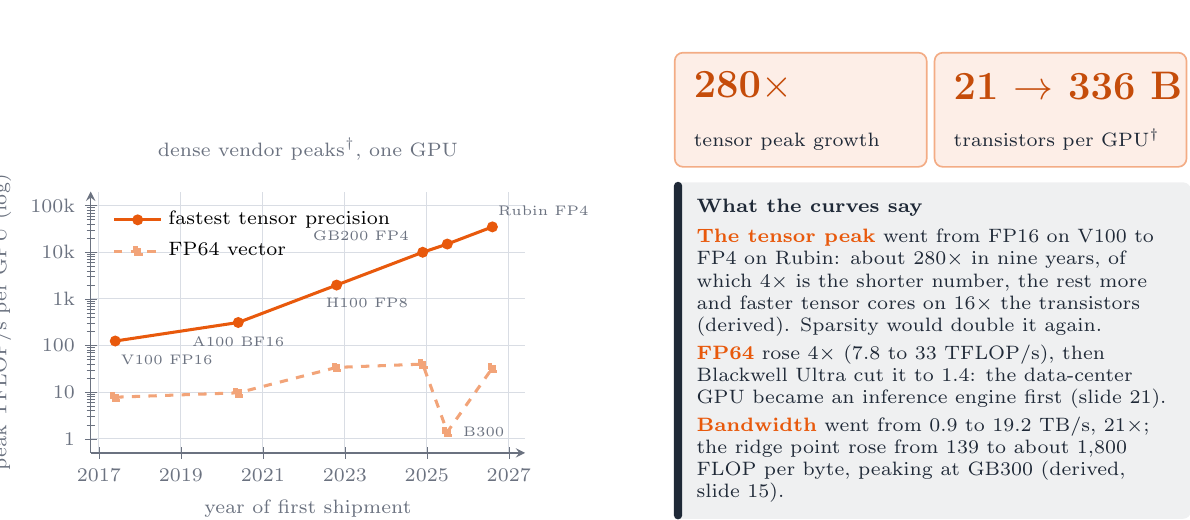
\begin{tikzpicture}
  \useasboundingbox (0,0) rectangle (14.4,5.9);
  \begin{scope}[shift={(0.8,0.5)}]
  \begin{axis}[lecture,width=7.1cm,height=4.9cm,ymode=log,xmin=2016.8,xmax=2027.4,ymin=0.5,ymax=200000,
      xlabel={year of first shipment},ylabel={peak TFLOP/s per GPU (log)},
      xtick={2017,2019,2021,2023,2025,2027},xticklabel style={/pgf/number format/1000 sep={}},scaled x ticks=false,
      ytick={1,10,100,1000,10000,100000},yticklabels={1,10,100,1k,10k,100k},
      legend style={at={(0.03,0.97)},anchor=north west},
      title style={font=\scriptsize,text=muted,at={(0.5,1.02)}},title={dense vendor peaks$^\dagger$, one GPU}]
    \addplot[attn,line width=1.1pt,mark=*,mark size=1.4pt] coordinates {(2017.4,125) (2020.4,312) (2022.8,1979) (2024.9,10000) (2025.5,15000) (2026.6,35000)};
    \addlegendentry{fastest tensor precision}
    \addplot[attn!55,line width=1.1pt,dashed,mark=square*,mark size=1.2pt] coordinates {(2017.4,7.8) (2020.4,9.7) (2022.8,34) (2024.9,40) (2025.5,1.4) (2026.6,33)};
    \addlegendentry{FP64 vector}
    \node[font=\tiny,text=muted,anchor=north west] at (axis cs:2017.3,100) {V100 FP16};
    \node[font=\tiny,text=muted,anchor=north] at (axis cs:2020.4,250) {A100 BF16};
    \node[font=\tiny,text=muted,anchor=north west] at (axis cs:2022.3,1700) {H100 FP8};
    \node[font=\tiny,text=muted,anchor=south east] at (axis cs:2024.8,11000) {GB200 FP4};
    \node[font=\tiny,text=muted,anchor=south west] at (axis cs:2026.5,38000) {Rubin FP4};
    \node[font=\tiny,text=muted,anchor=west] at (axis cs:2025.65,1.4) {B300};
  \end{axis}
  \end{scope}
  \stat{8.2}{5.6}{280$\times$}{tensor peak growth}{attn}
  \stat{11.5}{5.6}{21 $\to$ 336 B}{transistors per GPU$^\dagger$}{attn}
  \bgpanels{8.2}{3.95}{6.0cm}{What the curves say}{%
    \hl{attn}{The tensor peak} went from FP16 on V100 to FP4 on Rubin:
    about 280$\times$ in nine years, of which 4$\times$ is the shorter
    number, the rest more and faster tensor cores on 16$\times$ the
    transistors (derived). Sparsity would double it again.\\[2pt]
    \hl{attn}{FP64} rose 4$\times$ (7.8 to 33 TFLOP/s), then Blackwell
    Ultra cut it to 1.4: the data-center GPU became an inference
    engine first (slide 21).\\[2pt]
    \hl{attn}{Bandwidth} went from 0.9 to 19.2 TB/s, 21$\times$; the
    ridge point rose from 139 to about 1{,}800 FLOP per byte, peaking
    at GB300 (derived, slide 15).}
\end{tikzpicture}
\end{frame}

% ---------------------------------------------------------------- 3
\begin{frame}{The cadence: every two years, then every year}
\framesubtitle{Nine products in nine years; since 2024 the announced numbers have moved before shipment.}
\centering
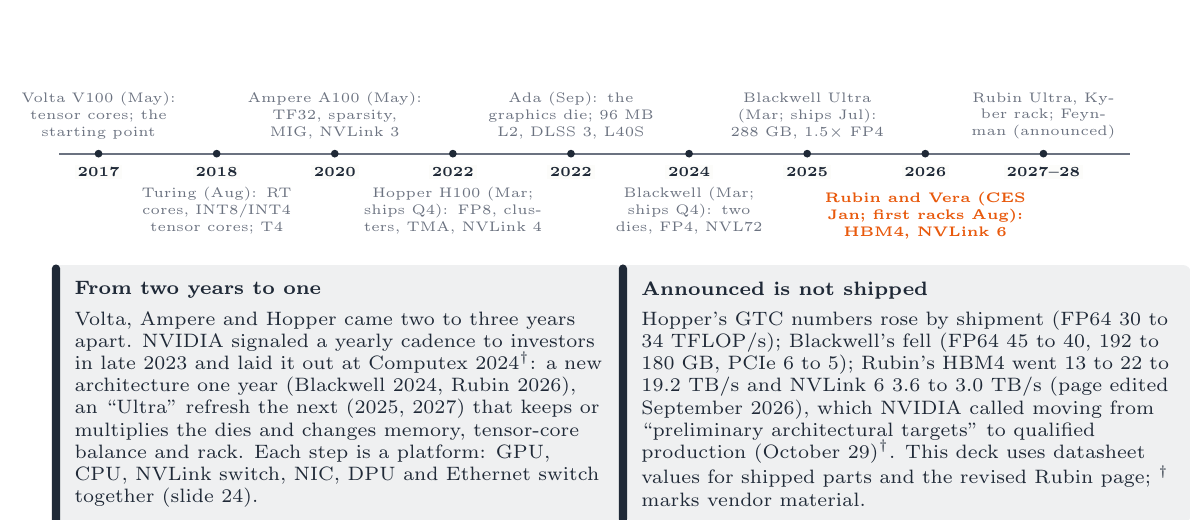
\begin{tikzpicture}
  \useasboundingbox (0,0) rectangle (14.4,5.9);
  \draw[muted,line width=0.8pt] (0.4,4.3) -- (14.0,4.3);
  \foreach \x in {0.9,2.4,3.9,5.4,6.9,8.4,9.9,11.4,12.9}{\fill[ink] (\x,4.3) circle (1.4pt);}
  \foreach \yr/\x in {2017/0.9,2018/2.4,2020/3.9,2022/5.4,2022/6.9,2024/8.4,2025/9.9,2026/11.4,2027--28/12.9}{
    \node[font=\tiny\bfseries,text=ink,fill=paper,inner sep=1pt] at (\x,4.07) {\yr};}
  \node[lab,anchor=south,text width=2.6cm,align=center,font=\tiny] at (0.9,4.43) {Volta V100 (May): tensor cores; the starting point};
  \node[lab,anchor=north,text width=2.6cm,align=center,font=\tiny] at (2.4,3.93) {Turing (Aug): RT cores, INT8/INT4 tensor cores; T4};
  \node[lab,anchor=south,text width=2.6cm,align=center,font=\tiny] at (3.9,4.43) {Ampere A100 (May): TF32, sparsity, MIG, NVLink 3};
  \node[lab,anchor=north,text width=2.6cm,align=center,font=\tiny] at (5.4,3.93) {Hopper H100 (Mar; ships Q4): FP8, clusters, TMA, NVLink 4};
  \node[lab,anchor=south,text width=2.6cm,align=center,font=\tiny] at (6.9,4.43) {Ada (Sep): the graphics die; 96 MB L2, DLSS 3, L40S};
  \node[lab,anchor=north,text width=2.6cm,align=center,font=\tiny] at (8.4,3.93) {Blackwell (Mar; ships Q4): two dies, FP4, NVL72};
  \node[lab,anchor=south,text width=2.6cm,align=center,font=\tiny] at (9.9,4.43) {Blackwell Ultra (Mar; ships Jul): 288 GB, 1.5$\times$ FP4};
  \node[anchor=north,text width=2.6cm,align=center,font=\tiny\bfseries,text=attn] at (11.4,3.93) {Rubin and Vera (CES Jan; first racks Aug): HBM4, NVLink 6};
  \node[lab,anchor=south,text width=2.6cm,align=center,font=\tiny] at (12.9,4.43) {Rubin Ultra, Kyber rack; Feynman (announced)};
  \bgpanels{0.3}{2.9}{6.7cm}{From two years to one}{%
    Volta, Ampere and Hopper came two to three years apart. NVIDIA
    signaled a yearly cadence to investors in late 2023 and laid it
    out at Computex 2024$^\dagger$: a new architecture one year
    (Blackwell 2024, Rubin 2026), an ``Ultra'' refresh the next (2025,
    2027) that keeps or multiplies the dies and changes memory,
    tensor-core balance and rack. Each step is a platform: GPU, CPU,
    NVLink switch, NIC, DPU and Ethernet switch together (slide 24).}
  \bgpanels{7.5}{2.9}{6.7cm}{Announced is not shipped}{%
    Hopper's GTC numbers rose by shipment (FP64 30 to 34 TFLOP/s);
    Blackwell's fell (FP64 45 to 40, 192 to 180 GB, PCIe 6 to 5);
    Rubin's HBM4 went 13 to 22 to 19.2 TB/s and NVLink 6 3.6 to 3.0
    TB/s (page edited September 2026), which NVIDIA called moving from
    ``preliminary architectural targets'' to qualified production
    (October 29)$^\dagger$. This deck uses datasheet values for shipped
    parts and the revised Rubin page; $^\dagger$ marks vendor material.}
\end{tikzpicture}
\end{frame}

% ---------------------------------------------------------------- 4
\stage{2}
\begin{frame}{Turing TU102 (2018): ray tracing and integer tensor cores}
\framesubtitle{A graphics die that carried Volta's SM into consumer GPUs and added two fixed-function units beside it.}
\centering
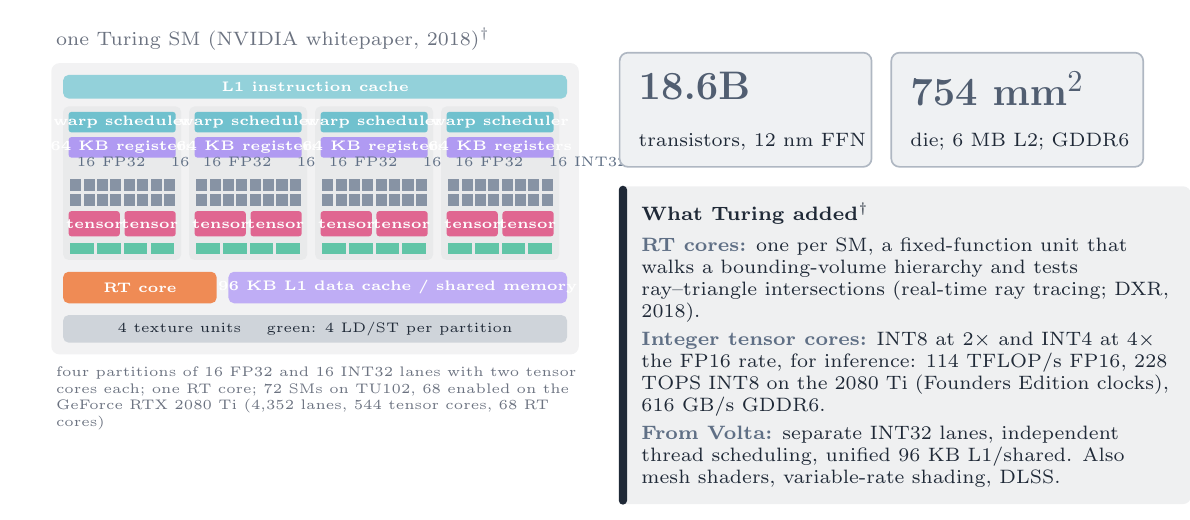
\begin{tikzpicture}
  \useasboundingbox (0,0) rectangle (14.4,5.9);
  \node[lab,anchor=south west] at (0.3,5.55) {one Turing SM (NVIDIA whitepaper, 2018)$^\dagger$};
  \begin{scope}[shift={(0.3,1.75)}]
    \fill[ink!6,rounded corners=3pt] (0,0) rectangle (6.7,3.7);
    \fill[vc!45,rounded corners=2pt] (0.15,3.25) rectangle (6.55,3.55); \node[font=\tiny\bfseries,text=white] at (3.35,3.4) {L1 instruction cache};
    \foreach \q in {0,...,3}{
      \begin{scope}[shift={(0.15+\q*1.6,1.2)}]
        \fill[ink!10,rounded corners=2pt] (0,0) rectangle (1.5,1.95);
        \fill[vc!60,rounded corners=1pt] (0.07,1.62) rectangle (1.43,1.88); \node[font=\fontsize{4.5}{5}\selectfont\bfseries,text=white] at (0.75,1.75) {warp scheduler};
        \fill[posc!55,rounded corners=1pt] (0.07,1.3) rectangle (1.43,1.56); \node[font=\fontsize{4.5}{5}\selectfont\bfseries,text=white] at (0.75,1.43) {64 KB registers};
        \foreach \r in {0,1}{\foreach \c in {0,...,7}{\fill[tok!75] (0.09+\c*0.17,0.88-\r*0.19) rectangle ++(0.14,0.15);}}
        \node[font=\fontsize{4.5}{5}\selectfont,text=tok,anchor=south west] at (0.05,1.06) {16 FP32 \quad 16 INT32};
        \fill[outc!75,rounded corners=1pt] (0.07,0.3) rectangle (0.72,0.62); \fill[outc!75,rounded corners=1pt] (0.78,0.3) rectangle (1.43,0.62);
        \node[font=\fontsize{4.5}{5}\selectfont\bfseries,text=white] at (0.4,0.46) {tensor}; \node[font=\fontsize{4.5}{5}\selectfont\bfseries,text=white] at (1.1,0.46) {tensor};
        \foreach \c in {0,...,3}{\fill[emb!65] (0.09+\c*0.34,0.07) rectangle ++(0.3,0.15);}
      \end{scope}}
    \fill[attn!70,rounded corners=2pt] (0.15,0.65) rectangle (2.1,1.05); \node[font=\tiny\bfseries,text=white] at (1.125,0.85) {RT core};
    \fill[posc!45,rounded corners=2pt] (2.25,0.65) rectangle (6.55,1.05); \node[font=\tiny\bfseries,text=white] at (4.4,0.85) {96 KB L1 data cache / shared memory};
    \fill[tok!30,rounded corners=2pt] (0.15,0.15) rectangle (6.55,0.5); \node[font=\tiny,text=ink] at (3.35,0.325) {4 texture units \quad green: 4 LD/ST per partition};
  \end{scope}
  \node[lab,font=\tiny,anchor=north west,text width=6.7cm] at (0.3,1.65) {four partitions of 16 FP32 and 16 INT32 lanes with two tensor cores each; one RT core; 72 SMs on TU102, 68 enabled on the GeForce RTX 2080 Ti (4{,}352 lanes, 544 tensor cores, 68 RT cores)};
  \stat{7.5}{5.6}{18.6B}{transistors, 12 nm FFN}{tok}
  \stat{10.95}{5.6}{754 mm$^2$}{die; 6 MB L2; GDDR6}{tok}
  \bgpanels{7.5}{3.9}{6.7cm}{What Turing added$^\dagger$}{%
    \hl{tok}{RT cores:} one per SM, a fixed-function unit that walks a
    bounding-volume hierarchy and tests ray--triangle intersections
    (real-time ray tracing; DXR, 2018).\\[2pt]
    \hl{tok}{Integer tensor cores:} INT8 at 2$\times$ and INT4 at
    4$\times$ the FP16 rate, for inference: 114 TFLOP/s FP16, 228 TOPS
    INT8 on the 2080 Ti (Founders Edition clocks), 616 GB/s GDDR6.\\[2pt]
    \hl{tok}{From Volta:} separate INT32 lanes, independent thread
    scheduling, unified 96 KB L1/shared. Also mesh shaders,
    variable-rate shading, DLSS.}
\end{tikzpicture}
\end{frame}

% ---------------------------------------------------------------- 5
\begin{frame}{The T4: inference at 70 watts, and tensor cores in every game}
\framesubtitle{Turing's data-center part was a low-profile PCIe card; its consumer part ran a neural network on every frame.}
\centering
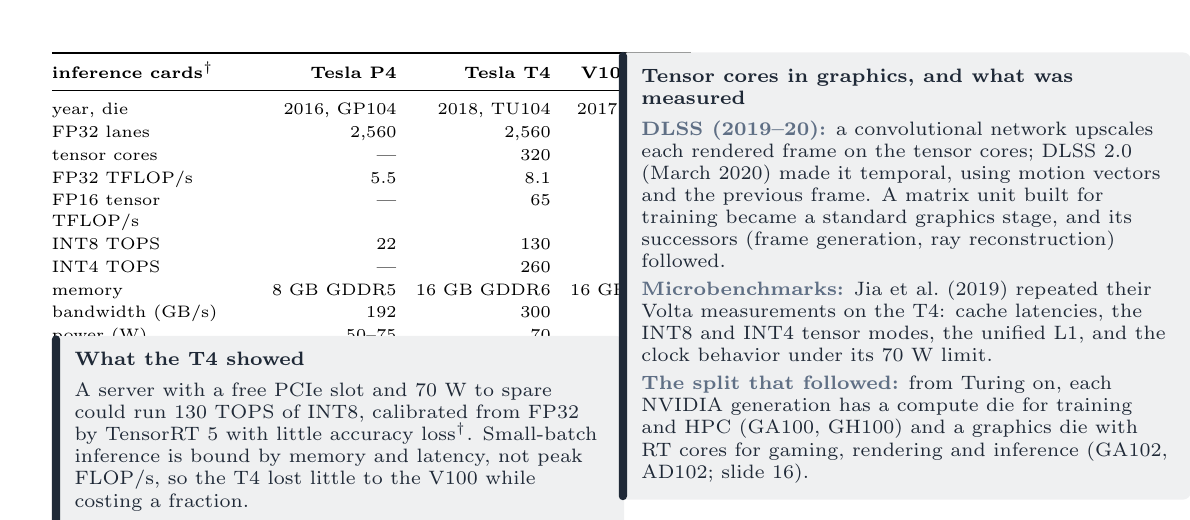
\begin{tikzpicture}
  \useasboundingbox (0,0) rectangle (14.4,5.9);
  \node[anchor=north west,inner sep=0,font=\fontsize{6.4}{7.6}\selectfont] at (0.3,5.6) {%
    \renewcommand{\arraystretch}{1.08}\setlength{\tabcolsep}{3.5pt}%
    \begin{tabular}{@{}>{\raggedright\arraybackslash}p{2.55cm}rrr@{}}
      \toprule
      \textbf{inference cards}$^\dagger$ & \textbf{Tesla P4} & \textbf{Tesla T4} & \textbf{V100 PCIe}\\
      \midrule
      year, die & 2016, GP104 & 2018, TU104 & 2017, GV100\\
      FP32 lanes & 2{,}560 & 2{,}560 & 5{,}120\\
      tensor cores & --- & 320 & 640\\
      FP32 TFLOP/s & 5.5 & 8.1 & 14\\
      FP16 tensor TFLOP/s & --- & 65 & 112\\
      INT8 TOPS & 22 & 130 & ---\\
      INT4 TOPS & --- & 260 & ---\\
      memory & 8 GB GDDR5 & 16 GB GDDR6 & 16 GB HBM2\\
      bandwidth (GB/s) & 192 & 300 & 900\\
      power (W) & 50--75 & 70 & 250\\
      \bottomrule
    \end{tabular}};
  \bgpanels{0.3}{2.0}{6.7cm}{What the T4 showed}{%
    A server with a free PCIe slot and 70 W to spare could run 130
    TOPS of INT8, calibrated from FP32 by TensorRT 5 with little
    accuracy loss$^\dagger$. Small-batch inference is bound by memory
    and latency, not peak FLOP/s, so the T4 lost little to the V100
    while costing a fraction.}
  \bgpanels{7.5}{5.6}{6.7cm}{Tensor cores in graphics, and what was measured}{%
    \hl{tok}{DLSS (2019--20):} a convolutional network upscales each
    rendered frame on the tensor cores; DLSS 2.0 (March 2020) made it
    temporal, using motion vectors and the previous frame. A matrix
    unit built for training became a standard graphics stage, and
    its successors (frame generation, ray reconstruction) followed.\\[2pt]
    \hl{tok}{Microbenchmarks:} Jia et al.\ (2019) repeated their Volta
    measurements on the T4: cache latencies, the INT8 and INT4 tensor
    modes, the unified L1, and the clock behavior under its 70 W
    limit.\\[2pt]
    \hl{tok}{The split that followed:} from Turing on, each NVIDIA
    generation has a compute die for training and HPC (GA100, GH100)
    and a graphics die with RT cores for gaming, rendering and
    inference (GA102, AD102; slide 16).}
\end{tikzpicture}
\end{frame}

% ---------------------------------------------------------------- 6
\stage{3}
\begin{frame}{Ampere GA100 (2020): the A100 die}
\framesubtitle{May 14, 2020: 54.2B transistors on TSMC 7 nm, 108 of 128 SMs enabled, 40 MB of L2, HBM2 at 1.6 TB/s.}
\centering
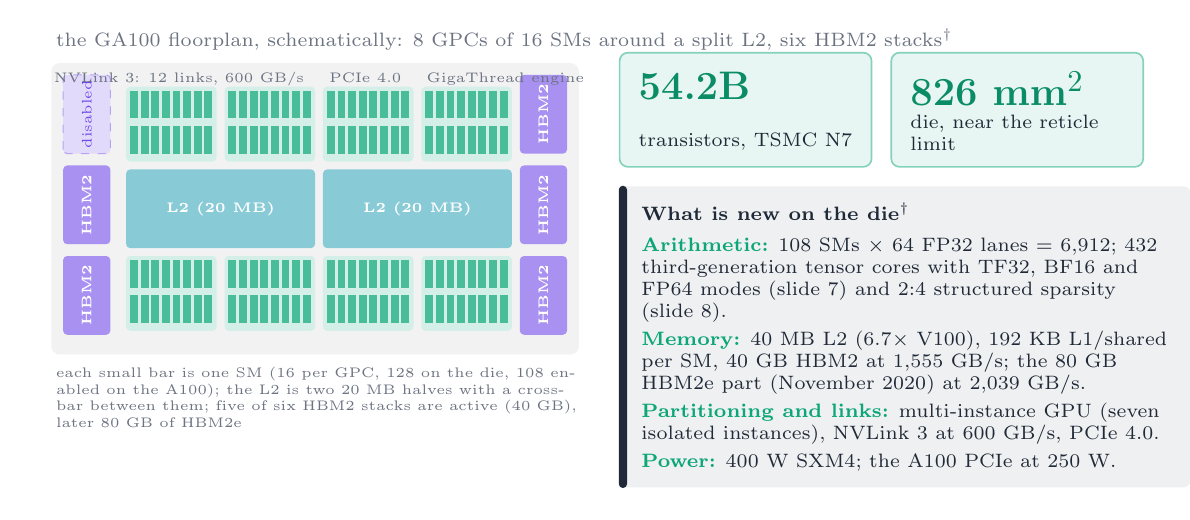
\begin{tikzpicture}
  \useasboundingbox (0,0) rectangle (14.4,5.9);
  \node[lab,anchor=south west] at (0.3,5.55) {the GA100 floorplan, schematically: 8 GPCs of 16 SMs around a split L2, six HBM2 stacks$^\dagger$};
  \begin{scope}[shift={(0.3,1.75)}]
    \fill[ink!6,rounded corners=3pt] (0,0) rectangle (6.7,3.7);
    % HBM stacks left and right (3 each; one disabled)
    \foreach \s in {0,1,2}{
      \pgfmathtruncatemacro{\on}{(\s==2)?0:1}
      \ifnum\on=1 \fill[posc!60,rounded corners=1.5pt] (0.15,0.25+\s*1.15) rectangle ++(0.6,1.0); \node[font=\fontsize{4.5}{5}\selectfont\bfseries,text=white,rotate=90] at (0.45,0.75+\s*1.15) {HBM2};
      \else \fill[posc!20,rounded corners=1.5pt,draw=posc!50,dashed,line width=0.4pt] (0.15,0.25+\s*1.15) rectangle ++(0.6,1.0); \node[font=\fontsize{4.5}{5}\selectfont,text=posc,rotate=90] at (0.45,0.75+\s*1.15) {disabled};\fi
      \fill[posc!60,rounded corners=1.5pt] (5.95,0.25+\s*1.15) rectangle ++(0.6,1.0); \node[font=\fontsize{4.5}{5}\selectfont\bfseries,text=white,rotate=90] at (6.25,0.75+\s*1.15) {HBM2};}
    % 8 GPCs: 4 top, 4 bottom; L2 halves in the middle
    \foreach \g in {0,...,3}{
      \foreach \row/\y in {0/2.45, 1/0.3}{
        \fill[emb!18,rounded corners=1.5pt] (0.95+\g*1.25,\y) rectangle ++(1.15,0.95);
        \foreach \r in {0,1}{\foreach \c in {0,...,7}{\fill[emb!75] (1.0+\g*1.25+\c*0.135,\y+0.55-\r*0.45) rectangle ++(0.1,0.35);}}}}
    \fill[vc!50,rounded corners=1.5pt] (0.95,1.35) rectangle (3.35,2.35); \node[font=\tiny\bfseries,text=white] at (2.15,1.85) {L2 (20 MB)};
    \fill[vc!50,rounded corners=1.5pt] (3.45,1.35) rectangle (5.85,2.35); \node[font=\tiny\bfseries,text=white] at (4.65,1.85) {L2 (20 MB)};
    \node[font=\fontsize{4.5}{5}\selectfont,text=muted] at (3.4,3.5) {NVLink 3: 12 links, 600 GB/s \quad PCIe 4.0 \quad GigaThread engine};
  \end{scope}
  \node[lab,font=\tiny,anchor=north west,text width=6.7cm] at (0.3,1.65) {each small bar is one SM (16 per GPC, 128 on the die, 108 enabled on the A100); the L2 is two 20 MB halves with a crossbar between them; five of six HBM2 stacks are active (40 GB), later 80 GB of HBM2e};
  \stat{7.5}{5.6}{54.2B}{transistors, TSMC N7}{emb}
  \stat{10.95}{5.6}{826 mm$^2$}{die, near the reticle limit}{emb}
  \bgpanels{7.5}{3.9}{6.7cm}{What is new on the die$^\dagger$}{%
    \hl{emb}{Arithmetic:} 108 SMs $\times$ 64 FP32 lanes $=$ 6{,}912;
    432 third-generation tensor cores with TF32, BF16 and FP64 modes
    (slide 7) and 2:4 structured sparsity (slide 8).\\[2pt]
    \hl{emb}{Memory:} 40 MB L2 (6.7$\times$ V100), 192 KB L1/shared
    per SM, 40 GB HBM2 at 1{,}555 GB/s; the 80 GB HBM2e part
    (November 2020) at 2{,}039 GB/s.\\[2pt]
    \hl{emb}{Partitioning and links:} multi-instance GPU (seven
    isolated instances), NVLink 3 at 600 GB/s, PCIe 4.0.\\[2pt]
    \hl{emb}{Power:} 400 W SXM4; the A100 PCIe at 250 W.}
\end{tikzpicture}
\end{frame}

% ---------------------------------------------------------------- 7
\begin{frame}{The A100 SM and the third-generation tensor core}
\framesubtitle{Twice Volta's matrix rate per SM per clock, with new input formats: TF32 for free, BF16, and FP64 on the tensor cores.}
\centering
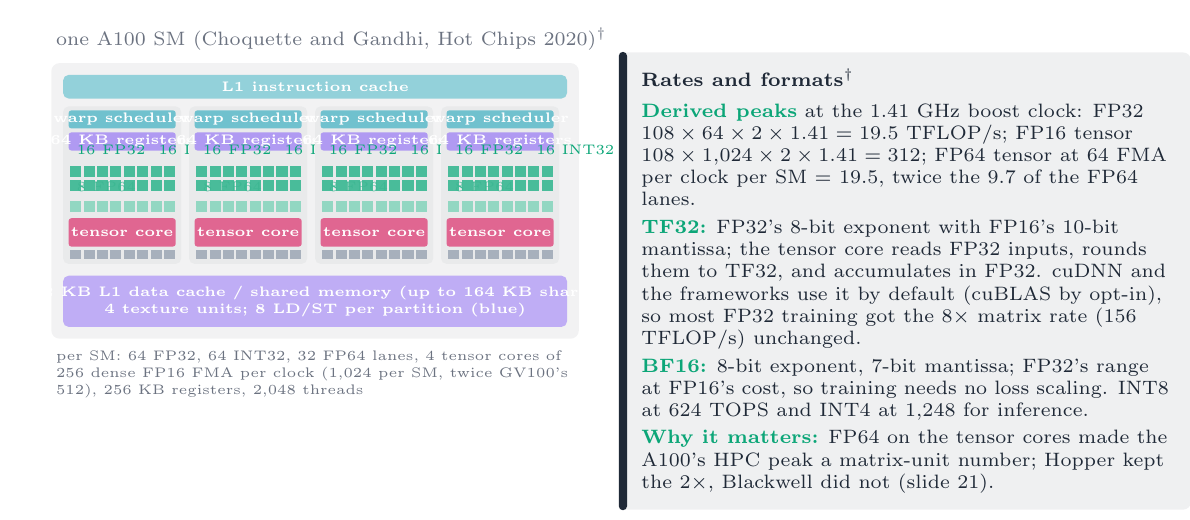
\begin{tikzpicture}
  \useasboundingbox (0,0) rectangle (14.4,5.9);
  \node[lab,anchor=south west] at (0.3,5.55) {one A100 SM (Choquette and Gandhi, Hot Chips 2020)$^\dagger$};
  \begin{scope}[shift={(0.3,1.95)}]
    \fill[ink!6,rounded corners=3pt] (0,0) rectangle (6.7,3.5);
    \fill[vc!45,rounded corners=2pt] (0.15,3.05) rectangle (6.55,3.35); \node[font=\tiny\bfseries,text=white] at (3.35,3.2) {L1 instruction cache};
    \foreach \q in {0,...,3}{
      \begin{scope}[shift={(0.15+\q*1.6,0.95)}]
        \fill[ink!10,rounded corners=2pt] (0,0) rectangle (1.5,2.0);
        \fill[vc!60,rounded corners=1pt] (0.07,1.72) rectangle (1.43,1.95); \node[font=\fontsize{4.5}{5}\selectfont\bfseries,text=white] at (0.75,1.835) {warp scheduler};
        \fill[posc!55,rounded corners=1pt] (0.07,1.44) rectangle (1.43,1.67); \node[font=\fontsize{4.5}{5}\selectfont\bfseries,text=white] at (0.75,1.555) {64 KB registers};
        \foreach \c in {0,...,7}{\fill[emb!75] (0.09+\c*0.17,1.1) rectangle ++(0.14,0.14);} \foreach \c in {0,...,7}{\fill[emb!75] (0.09+\c*0.17,0.92) rectangle ++(0.14,0.14);}
        \node[font=\fontsize{4.5}{5}\selectfont,text=emb,anchor=south west] at (0.05,1.26) {16 FP32 \ 16 INT32};
        \foreach \c in {0,...,7}{\fill[emb!45] (0.09+\c*0.17,0.66) rectangle ++(0.14,0.14);}
        \node[font=\fontsize{4.5}{5}\selectfont,text=emb!80,anchor=south west] at (0.05,0.80) {8 FP64};
        \fill[outc!75,rounded corners=1pt] (0.07,0.22) rectangle (1.43,0.58); \node[font=\fontsize{4.5}{5}\selectfont\bfseries,text=white] at (0.75,0.4) {tensor core};
        \foreach \c in {0,...,7}{\fill[tok!55] (0.09+\c*0.17,0.06) rectangle ++(0.14,0.12);}
      \end{scope}}
    \fill[posc!45,rounded corners=2pt] (0.15,0.15) rectangle (6.55,0.8); \node[font=\tiny\bfseries,text=white,align=center] at (3.35,0.475) {192 KB L1 data cache / shared memory (up to 164 KB shared)\\4 texture units; 8 LD/ST per partition (blue)};
  \end{scope}
  \node[lab,font=\tiny,anchor=north west,text width=6.7cm] at (0.3,1.85) {per SM: 64 FP32, 64 INT32, 32 FP64 lanes, 4 tensor cores of 256 dense FP16 FMA per clock (1{,}024 per SM, twice GV100's 512), 256 KB registers, 2{,}048 threads};
  \bgpanels{7.5}{5.6}{6.7cm}{Rates and formats$^\dagger$}{%
    \hl{emb}{Derived peaks} at the 1.41 GHz boost clock: FP32 $108
    \times 64 \times 2 \times 1.41 = 19.5$ TFLOP/s; FP16 tensor $108
    \times 1{,}024 \times 2 \times 1.41 = 312$; FP64 tensor at 64 FMA
    per clock per SM $=$ 19.5, twice the 9.7 of the FP64 lanes.\\[2pt]
    \hl{emb}{TF32:} FP32's 8-bit exponent with FP16's 10-bit mantissa;
    the tensor core reads FP32 inputs, rounds them to TF32, and
    accumulates in FP32. cuDNN and the frameworks use it by default
    (cuBLAS by opt-in), so most FP32 training got the 8$\times$ matrix
    rate (156 TFLOP/s) unchanged.\\[2pt]
    \hl{emb}{BF16:} 8-bit exponent, 7-bit mantissa; FP32's range at
    FP16's cost, so training needs no loss scaling. INT8 at 624 TOPS
    and INT4 at 1{,}248 for inference.\\[2pt]
    \hl{emb}{Why it matters:} FP64 on the tensor cores made the
    A100's HPC peak a matrix-unit number; Hopper kept the 2$\times$,
    Blackwell did not (slide 21).}
\end{tikzpicture}
\end{frame}

% ---------------------------------------------------------------- 8
\begin{frame}{Sparsity, multi-instance GPU, and the A100 memory system}
\framesubtitle{Three features for the data center: a 2$\times$ from pruned weights, seven GPUs in one, and a bigger, smarter L2.}
\centering
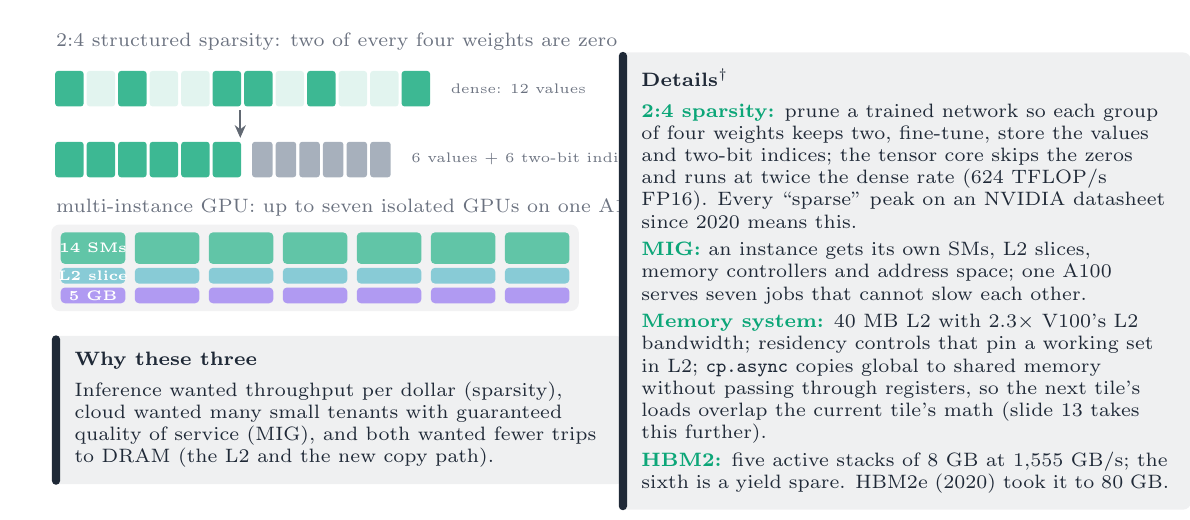
\begin{tikzpicture}
  \useasboundingbox (0,0) rectangle (14.4,5.9);
  \node[lab,anchor=south west] at (0.3,5.55) {2:4 structured sparsity: two of every four weights are zero};
  \begin{scope}[shift={(0.3,4.35)}]
    \foreach \i/\v in {0/0.9,1/0,2/0.4,3/0,4/0,5/0.7,6/0.3,7/0,8/0.5,9/0,10/0,11/0.8}{
      \pgfmathtruncatemacro{\sh}{(\v>0)?80:12}
      \fill[emb!\sh,rounded corners=1pt] (0.05+\i*0.4,0.55) rectangle ++(0.36,0.45);}
    \node[font=\tiny,text=muted,anchor=west] at (4.95,0.78) {dense: 12 values};
    \draw[flow] (2.4,0.5) -- (2.4,0.15);
    \foreach \i in {0,...,5}{\fill[emb!80,rounded corners=1pt] (0.05+\i*0.4,-0.35) rectangle ++(0.36,0.45);}
    \foreach \i in {0,...,5}{\fill[tok!55,rounded corners=1pt] (2.55+\i*0.3,-0.35) rectangle ++(0.26,0.45);}
    \node[font=\tiny,text=muted,anchor=west] at (4.45,-0.12) {6 values $+$ 6 two-bit indices};
  \end{scope}
  \node[lab,anchor=south west] at (0.3,3.45) {multi-instance GPU: up to seven isolated GPUs on one A100};
  \begin{scope}[shift={(0.3,2.3)}]
    \fill[ink!6,rounded corners=3pt] (0,0) rectangle (6.7,1.1);
    \foreach \i in {0,...,6}{
      \fill[emb!65,rounded corners=1.5pt] (0.12+\i*0.94,0.6) rectangle ++(0.82,0.4);
      \fill[vc!50,rounded corners=1.5pt] (0.12+\i*0.94,0.35) rectangle ++(0.82,0.2);
      \fill[posc!55,rounded corners=1.5pt] (0.12+\i*0.94,0.1) rectangle ++(0.82,0.2);}
    \node[font=\fontsize{4.5}{5}\selectfont\bfseries,text=white] at (0.53,0.8) {14 SMs}; \node[font=\fontsize{4.5}{5}\selectfont\bfseries,text=white] at (0.53,0.45) {L2 slice}; \node[font=\fontsize{4.5}{5}\selectfont\bfseries,text=white] at (0.53,0.2) {5 GB};
  \end{scope}
  \bgpanels{0.3}{2.0}{6.7cm}{Why these three}{%
    Inference wanted throughput per dollar (sparsity), cloud wanted
    many small tenants with guaranteed quality of service (MIG), and
    both wanted fewer trips to DRAM (the L2 and the new copy path).}
  \bgpanels{7.5}{5.6}{6.7cm}{Details$^\dagger$}{%
    \hl{emb}{2:4 sparsity:} prune a trained network so each group of
    four weights keeps two, fine-tune, store the values and two-bit
    indices; the tensor core skips the zeros and runs at twice the
    dense rate (624 TFLOP/s FP16). Every ``sparse'' peak on an NVIDIA
    datasheet since 2020 means this.\\[2pt]
    \hl{emb}{MIG:} an instance gets its own SMs, L2 slices, memory
    controllers and address space; one A100 serves seven jobs that
    cannot slow each other.\\[2pt]
    \hl{emb}{Memory system:} 40 MB L2 with 2.3$\times$ V100's L2
    bandwidth; residency controls that pin a working set in L2;
    \texttt{cp.async} copies global to shared memory without passing
    through registers, so the next tile's loads overlap the current
    tile's math (slide 13 takes this further).\\[2pt]
    \hl{emb}{HBM2:} five active stacks of 8 GB at 1{,}555 GB/s; the
    sixth is a yield spare. HBM2e (2020) took it to 80 GB.}
\end{tikzpicture}
\end{frame}

% ---------------------------------------------------------------- 9
\begin{frame}{Ampere deployed: DGX A100, early systems, and GA102}
\framesubtitle{Eight A100s behind six NVSwitches became the unit of AI infrastructure; the graphics die went its own way.}
\centering
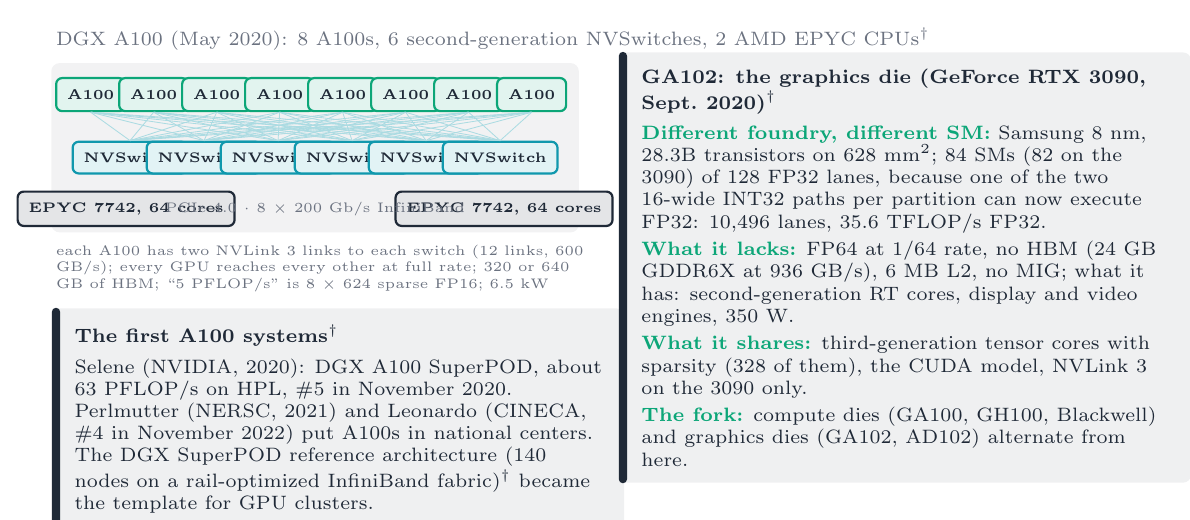
\begin{tikzpicture}
  \useasboundingbox (0,0) rectangle (14.4,5.9);
  \node[lab,anchor=south west] at (0.3,5.55) {DGX A100 (May 2020): 8 A100s, 6 second-generation NVSwitches, 2 AMD EPYC CPUs$^\dagger$};
  \begin{scope}[shift={(0.3,3.3)}]
    \fill[ink!6,rounded corners=3pt] (0,0) rectangle (6.7,2.15);
    \foreach \g in {0,...,7}{\node[comp=emb,minimum width=0.62cm,minimum height=0.42cm,font=\fontsize{4.5}{5}\selectfont\bfseries,text=ink] (a\g) at (0.5+\g*0.8,1.75) {A100};}
    \foreach \s in {0,...,5}{\node[comp=vc,minimum width=0.72cm,minimum height=0.36cm,font=\fontsize{4.5}{5}\selectfont\bfseries,text=ink] (n\s) at (1.0+\s*0.94,0.95) {NVSwitch};}
    \foreach \g in {0,...,7}{\foreach \s in {0,...,5}{\draw[vc!35,line width=0.3pt] (a\g.south) -- (n\s.north);}}
    \foreach \c/\x in {0/0.95,1/5.75}{\node[comp=ink,minimum width=1.35cm,minimum height=0.36cm,font=\fontsize{4.5}{5}\selectfont\bfseries,text=ink] (c\c) at (\x,0.3) {EPYC 7742, 64 cores};}
    \node[font=\fontsize{4.5}{5}\selectfont,text=muted] at (3.35,0.3) {PCIe 4.0 $\cdot$ 8 $\times$ 200 Gb/s InfiniBand};
  \end{scope}
  \node[lab,font=\tiny,anchor=north west,text width=6.7cm] at (0.3,3.2) {each A100 has two NVLink 3 links to each switch (12 links, 600 GB/s); every GPU reaches every other at full rate; 320 or 640 GB of HBM; ``5 PFLOP/s'' is 8 $\times$ 624 sparse FP16; 6.5 kW};
  \bgpanels{0.3}{2.35}{6.7cm}{The first A100 systems$^\dagger$}{%
    Selene (NVIDIA, 2020): DGX A100 SuperPOD, about 63 PFLOP/s on HPL,
    \#5 in November 2020. Perlmutter (NERSC, 2021) and Leonardo
    (CINECA, \#4 in November 2022) put A100s in national centers. The
    DGX SuperPOD reference architecture (140 nodes on a rail-optimized
    InfiniBand fabric)$^\dagger$ became the template for GPU clusters.}
  \bgpanels{7.5}{5.6}{6.7cm}{GA102: the graphics die (GeForce RTX 3090, Sept.\ 2020)$^\dagger$}{%
    \hl{emb}{Different foundry, different SM:} Samsung 8 nm, 28.3B
    transistors on 628 mm$^2$; 84 SMs (82 on the 3090) of 128 FP32
    lanes, because one of the two 16-wide INT32 paths per partition
    can now execute FP32: 10{,}496 lanes, 35.6 TFLOP/s FP32.\\[2pt]
    \hl{emb}{What it lacks:} FP64 at 1/64 rate, no HBM (24 GB GDDR6X
    at 936 GB/s), 6 MB L2, no MIG; what it has: second-generation RT
    cores, display and video engines, 350 W.\\[2pt]
    \hl{emb}{What it shares:} third-generation tensor cores with
    sparsity (328 of them), the CUDA model, NVLink 3 on the 3090
    only.\\[2pt]
    \hl{emb}{The fork:} compute dies (GA100, GH100, Blackwell) and
    graphics dies (GA102, AD102) alternate from here.}
\end{tikzpicture}
\end{frame}

% ---------------------------------------------------------------- 10
\begin{frame}{The precision ladder: FP32 to FP4}
\framesubtitle{Every format trades mantissa bits for throughput; below 8 bits a shared scale per block of values keeps the range.}
\centering
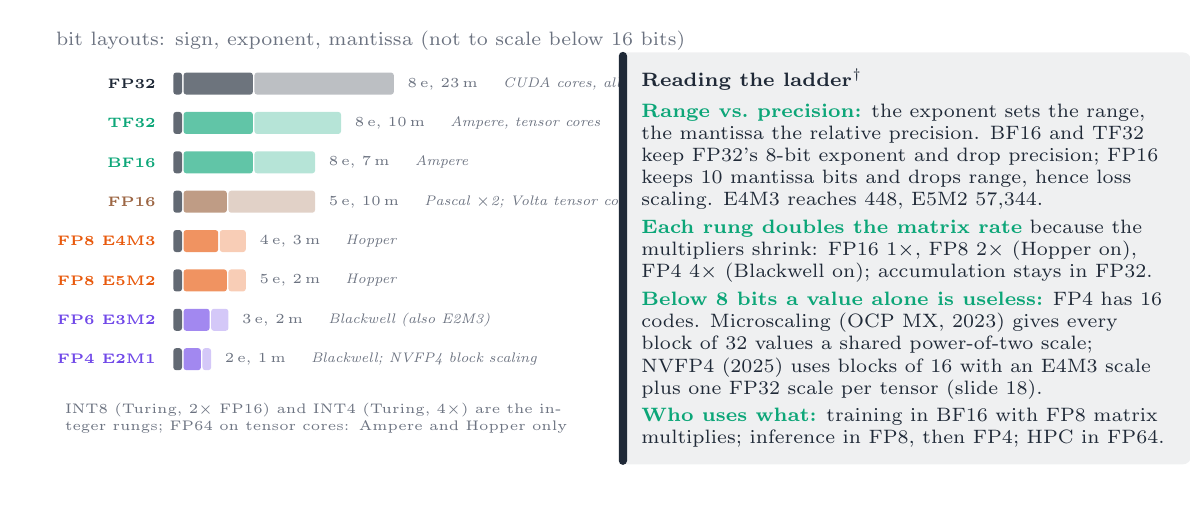
\begin{tikzpicture}
  \useasboundingbox (0,0) rectangle (14.4,5.9);
  \node[lab,anchor=south west] at (0.3,5.55) {bit layouts: sign, exponent, mantissa (not to scale below 16 bits)};
  \begin{scope}[shift={(0.3,0.75)}]
    \foreach \name/\s/\e/\m/\y/\gen/\c in {
        FP32/1/8/23/4.3/{CUDA cores, all}/ink,
        TF32/1/8/10/3.8/{Ampere, tensor cores}/emb,
        BF16/1/8/7/3.3/{Ampere}/emb,
        FP16/1/5/10/2.8/{Pascal $\times$2; Volta tensor cores}/trn,
        {FP8 E4M3}/1/4/3/2.3/{Hopper}/attn,
        {FP8 E5M2}/1/5/2/1.8/{Hopper}/attn,
        {FP6 E3M2}/1/3/2/1.3/{Blackwell (also E2M3)}/posc,
        {FP4 E2M1}/1/2/1/0.8/{Blackwell; NVFP4 block scaling}/posc}{
      \node[font=\tiny\bfseries,text=\c,anchor=east] at (1.45,\y+0.14) {\name};
      \pgfmathsetmacro{\we}{\e*0.11}\pgfmathsetmacro{\wm}{min(\m,12)*0.11+((\m>12)?0.45:0)}
      \fill[ink!70,rounded corners=1pt] (1.55,\y) rectangle ++(0.11,0.28);
      \fill[\c!65,rounded corners=1pt] (1.68,\y) rectangle ++(\we,0.28);
      \fill[\c!30,rounded corners=1pt] (1.7+\we,\y) rectangle ++(\wm,0.28);
      \node[font=\fontsize{4.5}{5}\selectfont,text=muted,anchor=west] at (1.75+\we+\wm,\y+0.14) {\e\,e, \m\,m \quad \textit{\gen}};}
    \node[font=\tiny,text=muted,anchor=north west,text width=6.5cm] at (0.05,0.5) {INT8 (Turing, 2$\times$ FP16) and INT4 (Turing, 4$\times$) are the integer rungs; FP64 on tensor cores: Ampere and Hopper only};
  \end{scope}
  \bgpanels{7.5}{5.6}{6.7cm}{Reading the ladder$^\dagger$}{%
    \hl{emb}{Range vs.\ precision:} the exponent sets the range, the
    mantissa the relative precision. BF16 and TF32 keep FP32's 8-bit
    exponent and drop precision; FP16 keeps 10 mantissa bits and
    drops range, hence loss scaling. E4M3 reaches 448, E5M2
    57{,}344.\\[2pt]
    \hl{emb}{Each rung doubles the matrix rate} because the
    multipliers shrink: FP16 1$\times$, FP8 2$\times$ (Hopper on), FP4
    4$\times$ (Blackwell on); accumulation stays in FP32.\\[2pt]
    \hl{emb}{Below 8 bits a value alone is useless:} FP4 has 16
    codes. Microscaling (OCP MX, 2023) gives every block of 32 values
    a shared power-of-two scale; NVFP4 (2025) uses blocks of 16 with
    an E4M3 scale plus one FP32 scale per tensor (slide 18).\\[2pt]
    \hl{emb}{Who uses what:} training in BF16 with FP8 matrix
    multiplies; inference in FP8, then FP4; HPC in FP64.}
\end{tikzpicture}
\end{frame}

% ---------------------------------------------------------------- 11
\stage{4}
\begin{frame}{Hopper GH100 (2022): the H100}
\framesubtitle{March 2022, shipping Q4 2022: 80B transistors on TSMC 4N, 132 of 144 SMs, HBM3 at 3.35 TB/s, 700 W.}
\centering
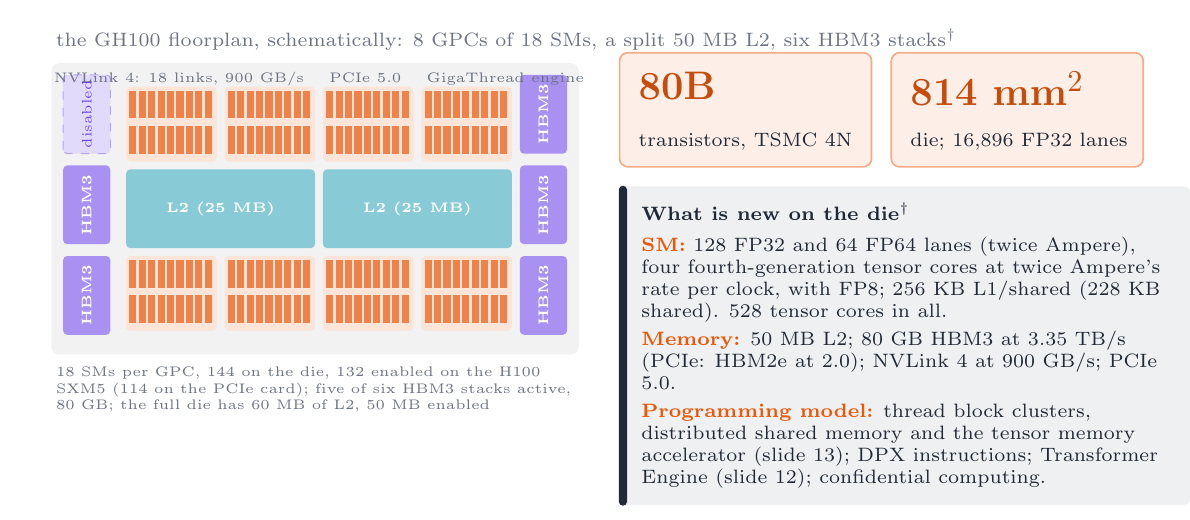
\begin{tikzpicture}
  \useasboundingbox (0,0) rectangle (14.4,5.9);
  \node[lab,anchor=south west] at (0.3,5.55) {the GH100 floorplan, schematically: 8 GPCs of 18 SMs, a split 50 MB L2, six HBM3 stacks$^\dagger$};
  \begin{scope}[shift={(0.3,1.75)}]
    \fill[ink!6,rounded corners=3pt] (0,0) rectangle (6.7,3.7);
    \foreach \s in {0,1,2}{
      \pgfmathtruncatemacro{\on}{(\s==2)?0:1}
      \ifnum\on=1 \fill[posc!60,rounded corners=1.5pt] (0.15,0.25+\s*1.15) rectangle ++(0.6,1.0); \node[font=\fontsize{4.5}{5}\selectfont\bfseries,text=white,rotate=90] at (0.45,0.75+\s*1.15) {HBM3};
      \else \fill[posc!20,rounded corners=1.5pt,draw=posc!50,dashed,line width=0.4pt] (0.15,0.25+\s*1.15) rectangle ++(0.6,1.0); \node[font=\fontsize{4.5}{5}\selectfont,text=posc,rotate=90] at (0.45,0.75+\s*1.15) {disabled};\fi
      \fill[posc!60,rounded corners=1.5pt] (5.95,0.25+\s*1.15) rectangle ++(0.6,1.0); \node[font=\fontsize{4.5}{5}\selectfont\bfseries,text=white,rotate=90] at (6.25,0.75+\s*1.15) {HBM3};}
    \foreach \g in {0,...,3}{
      \foreach \row/\y in {0/2.45, 1/0.3}{
        \fill[attn!16,rounded corners=1.5pt] (0.95+\g*1.25,\y) rectangle ++(1.15,0.95);
        \foreach \r in {0,1}{\foreach \c in {0,...,8}{\fill[attn!75] (0.99+\g*1.25+\c*0.12,\y+0.55-\r*0.45) rectangle ++(0.09,0.35);}}}}
    \fill[vc!50,rounded corners=1.5pt] (0.95,1.35) rectangle (3.35,2.35); \node[font=\tiny\bfseries,text=white] at (2.15,1.85) {L2 (25 MB)};
    \fill[vc!50,rounded corners=1.5pt] (3.45,1.35) rectangle (5.85,2.35); \node[font=\tiny\bfseries,text=white] at (4.65,1.85) {L2 (25 MB)};
    \node[font=\fontsize{4.5}{5}\selectfont,text=muted] at (3.4,3.5) {NVLink 4: 18 links, 900 GB/s \quad PCIe 5.0 \quad GigaThread engine};
  \end{scope}
  \node[lab,font=\tiny,anchor=north west,text width=6.7cm] at (0.3,1.65) {18 SMs per GPC, 144 on the die, 132 enabled on the H100 SXM5 (114 on the PCIe card); five of six HBM3 stacks active, 80 GB; the full die has 60 MB of L2, 50 MB enabled};
  \stat{7.5}{5.6}{80B}{transistors, TSMC 4N}{attn}
  \stat{10.95}{5.6}{814 mm$^2$}{die; 16{,}896 FP32 lanes}{attn}
  \bgpanels{7.5}{3.9}{6.7cm}{What is new on the die$^\dagger$}{%
    \hl{attn}{SM:} 128 FP32 and 64 FP64 lanes (twice Ampere), four
    fourth-generation tensor cores at twice Ampere's rate per clock,
    with FP8; 256 KB L1/shared (228 KB shared). 528 tensor cores in
    all.\\[2pt]
    \hl{attn}{Memory:} 50 MB L2; 80 GB HBM3 at 3.35 TB/s (PCIe: HBM2e
    at 2.0); NVLink 4 at 900 GB/s; PCIe 5.0.\\[2pt]
    \hl{attn}{Programming model:} thread block clusters, distributed
    shared memory and the tensor memory accelerator (slide 13); DPX
    instructions; Transformer Engine (slide 12); confidential
    computing.}
\end{tikzpicture}
\end{frame}

% ---------------------------------------------------------------- 12
\begin{frame}{Transformer Engine and FP8: the first 8-bit training format}
\framesubtitle{Two FP8 encodings, per-tensor scales from recent magnitudes, FP32 accumulation: twice the FP16 rate.}
\centering
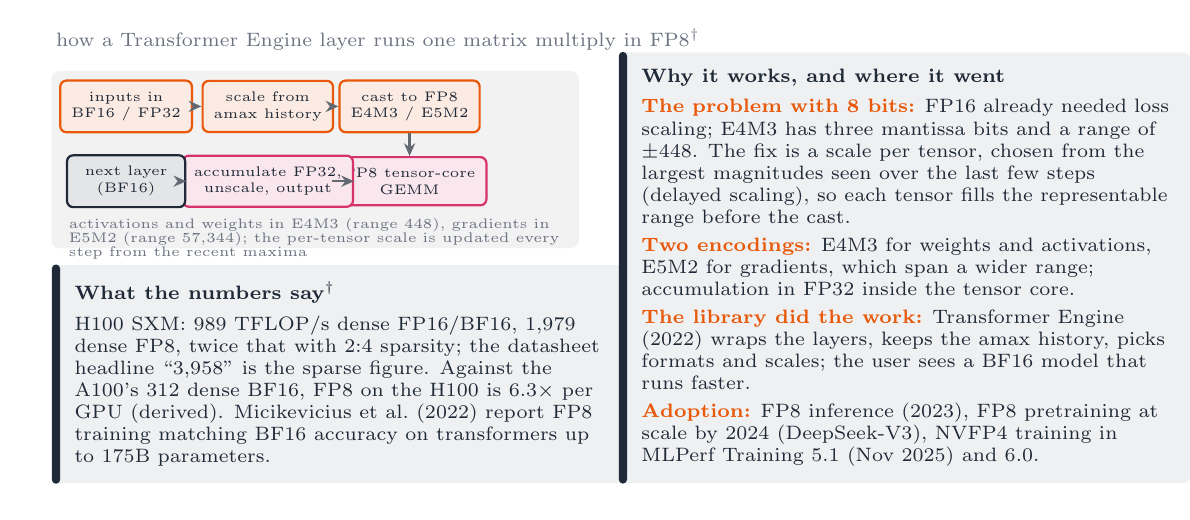
\begin{tikzpicture}
  \useasboundingbox (0,0) rectangle (14.4,5.9);
  \node[lab,anchor=south west] at (0.3,5.55) {how a Transformer Engine layer runs one matrix multiply in FP8$^\dagger$};
  \begin{scope}[shift={(0.3,3.1)}]
    \fill[ink!6,rounded corners=3pt] (0,0) rectangle (6.7,2.25);
    \node[comp=attn,minimum width=1.5cm,minimum height=0.55cm,font=\tiny,text=ink,align=center] (in) at (0.95,1.8) {inputs in\\BF16 / FP32};
    \node[comp=attn,minimum width=1.5cm,minimum height=0.55cm,font=\tiny,text=ink,align=center] (sc) at (2.75,1.8) {scale from\\amax history};
    \node[comp=attn,minimum width=1.5cm,minimum height=0.55cm,font=\tiny,text=ink,align=center] (cast) at (4.55,1.8) {cast to FP8\\E4M3 / E5M2};
    \node[comp=outc,minimum width=1.5cm,minimum height=0.55cm,font=\tiny,text=ink,align=center] (mma) at (4.55,0.85) {FP8 tensor-core\\GEMM};
    \node[comp=outc,minimum width=1.5cm,minimum height=0.55cm,font=\tiny,text=ink,align=center] (out) at (2.75,0.85) {accumulate FP32,\\unscale, output};
    \node[comp=ink,minimum width=1.5cm,minimum height=0.55cm,font=\tiny,text=ink,align=center] (nxt) at (0.95,0.85) {next layer\\(BF16)};
    \draw[flow] (in) -- (sc); \draw[flow] (sc) -- (cast); \draw[flow] (cast) -- (mma); \draw[flow] (mma) -- (out); \draw[flow] (out) -- (nxt);
    \node[font=\fontsize{4.5}{5}\selectfont,text=muted,anchor=north west,text width=6.5cm] at (0.1,0.5) {activations and weights in E4M3 (range 448), gradients in E5M2 (range 57{,}344); the per-tensor scale is updated every step from the recent maxima};
  \end{scope}
  \bgpanels{0.3}{2.9}{6.7cm}{What the numbers say$^\dagger$}{%
    H100 SXM: 989 TFLOP/s dense FP16/BF16, 1{,}979 dense FP8, twice
    that with 2:4 sparsity; the datasheet headline ``3{,}958'' is the
    sparse figure. Against the A100's 312 dense BF16, FP8 on the
    H100 is 6.3$\times$ per GPU (derived). Micikevicius et al.\
    (2022) report FP8 training matching BF16 accuracy on
    transformers up to 175B parameters.}
  \bgpanels{7.5}{5.6}{6.7cm}{Why it works, and where it went}{%
    \hl{attn}{The problem with 8 bits:} FP16 already needed loss
    scaling; E4M3 has three mantissa bits and a range of $\pm 448$.
    The fix is a scale per tensor, chosen from the largest magnitudes
    seen over the last few steps (delayed scaling), so each tensor
    fills the representable range before the cast.\\[2pt]
    \hl{attn}{Two encodings:} E4M3 for weights and activations, E5M2
    for gradients, which span a wider range; accumulation in FP32
    inside the tensor core.\\[2pt]
    \hl{attn}{The library did the work:} Transformer Engine (2022)
    wraps the layers, keeps the amax history, picks formats and
    scales; the user sees a BF16 model that runs faster.\\[2pt]
    \hl{attn}{Adoption:} FP8 inference (2023), FP8 pretraining at
    scale by 2024 (DeepSeek-V3), NVFP4 training in MLPerf Training
    5.1 (Nov 2025) and 6.0.}
\end{tikzpicture}
\end{frame}

% ---------------------------------------------------------------- 13
\begin{frame}{Clusters, distributed shared memory, and the TMA}
\framesubtitle{Hopper added a level between the block and the grid, and a copy engine that moves tiles while the SM computes.}
\centering
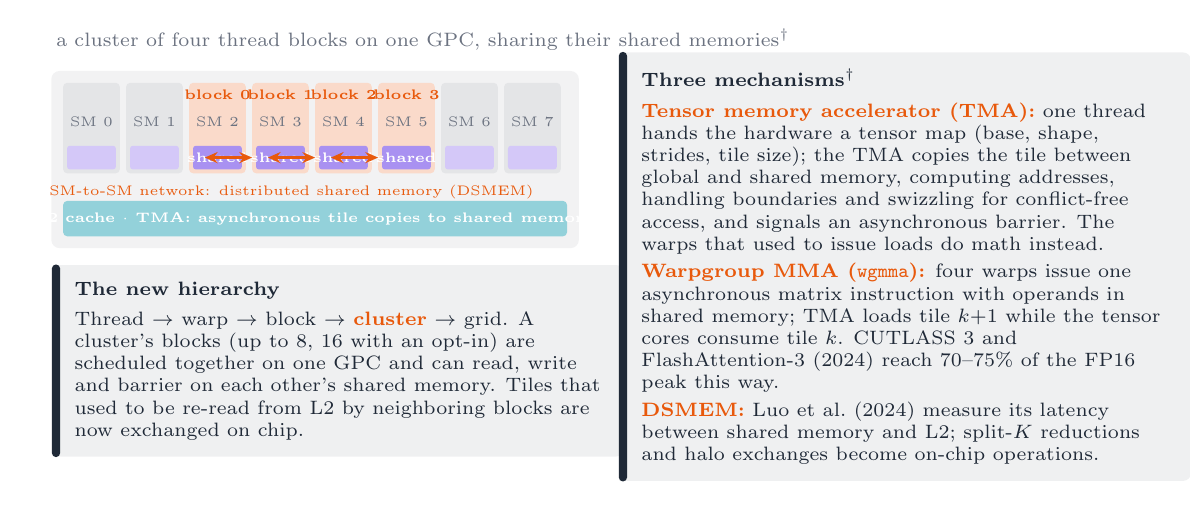
\begin{tikzpicture}
  \useasboundingbox (0,0) rectangle (14.4,5.9);
  \node[lab,anchor=south west] at (0.3,5.55) {a cluster of four thread blocks on one GPC, sharing their shared memories$^\dagger$};
  \begin{scope}[shift={(0.3,3.1)}]
    \fill[ink!6,rounded corners=3pt] (0,0) rectangle (6.7,2.25);
    \foreach \s in {0,...,7}{
      \pgfmathtruncatemacro{\inc}{(\s>=2 && \s<=5)?1:0}
      \ifnum\inc=1
        \fill[attn!22,rounded corners=1.5pt] (0.15+\s*0.8,0.95) rectangle ++(0.72,1.15);
        \fill[posc!60,rounded corners=1pt] (0.2+\s*0.8,1.0) rectangle ++(0.62,0.3); \node[font=\fontsize{4.5}{5}\selectfont\bfseries,text=white] at (0.51+\s*0.8,1.15) {shared};
        \node[font=\fontsize{4.5}{5}\selectfont\bfseries,text=attn] at (0.51+\s*0.8,1.95) {block \the\numexpr\s-2\relax};
      \else
        \fill[ink!12,rounded corners=1.5pt] (0.15+\s*0.8,0.95) rectangle ++(0.72,1.15);
        \fill[posc!30,rounded corners=1pt] (0.2+\s*0.8,1.0) rectangle ++(0.62,0.3);
      \fi
      \node[font=\fontsize{4.5}{5}\selectfont,text=muted] at (0.51+\s*0.8,1.6) {SM \s};}
    \draw[attn,line width=0.9pt,<->] (1.95,1.15) -- (2.55,1.15); \draw[attn,line width=0.9pt,<->] (2.75,1.15) -- (3.35,1.15); \draw[attn,line width=0.9pt,<->] (3.55,1.15) -- (4.15,1.15);
    \node[font=\fontsize{4.5}{5}\selectfont,text=attn,anchor=north] at (3.05,0.93) {SM-to-SM network: distributed shared memory (DSMEM)};
    \fill[vc!45,rounded corners=1.5pt] (0.15,0.15) rectangle (6.55,0.6); \node[font=\tiny\bfseries,text=white] at (3.35,0.375) {L2 cache $\cdot$ TMA: asynchronous tile copies to shared memory};
  \end{scope}
  \bgpanels{0.3}{2.9}{6.7cm}{The new hierarchy}{%
    Thread $\to$ warp $\to$ block $\to$ \hl{attn}{cluster} $\to$ grid.
    A cluster's blocks (up to 8, 16 with an opt-in) are scheduled
    together on one GPC and can read, write and barrier on each
    other's shared memory. Tiles that used to be re-read from L2 by
    neighboring blocks are now exchanged on chip.}
  \bgpanels{7.5}{5.6}{6.7cm}{Three mechanisms$^\dagger$}{%
    \hl{attn}{Tensor memory accelerator (TMA):} one thread hands the
    hardware a tensor map (base, shape, strides, tile size); the TMA
    copies the tile between global and shared memory, computing
    addresses, handling boundaries and swizzling for conflict-free
    access, and signals an asynchronous barrier. The warps that used
    to issue loads do math instead.\\[2pt]
    \hl{attn}{Warpgroup MMA (\texttt{wgmma}):} four warps issue one
    asynchronous matrix instruction with operands in shared memory;
    TMA loads tile $k{+}1$ while the tensor cores consume tile $k$.
    CUTLASS 3 and FlashAttention-3 (2024) reach 70--75\% of the FP16
    peak this way.\\[2pt]
    \hl{attn}{DSMEM:} Luo et al.\ (2024) measure its latency between
    shared memory and L2; split-$K$ reductions and halo exchanges
    become on-chip operations.}
\end{tikzpicture}
\end{frame}

% ---------------------------------------------------------------- 14
\begin{frame}{NVLink 4, NVSwitch 3, and the Grace Hopper superchip}
\framesubtitle{900 GB/s between GPUs, reductions in the switch, and a CPU joined to the GPU at memory speed.}
\centering
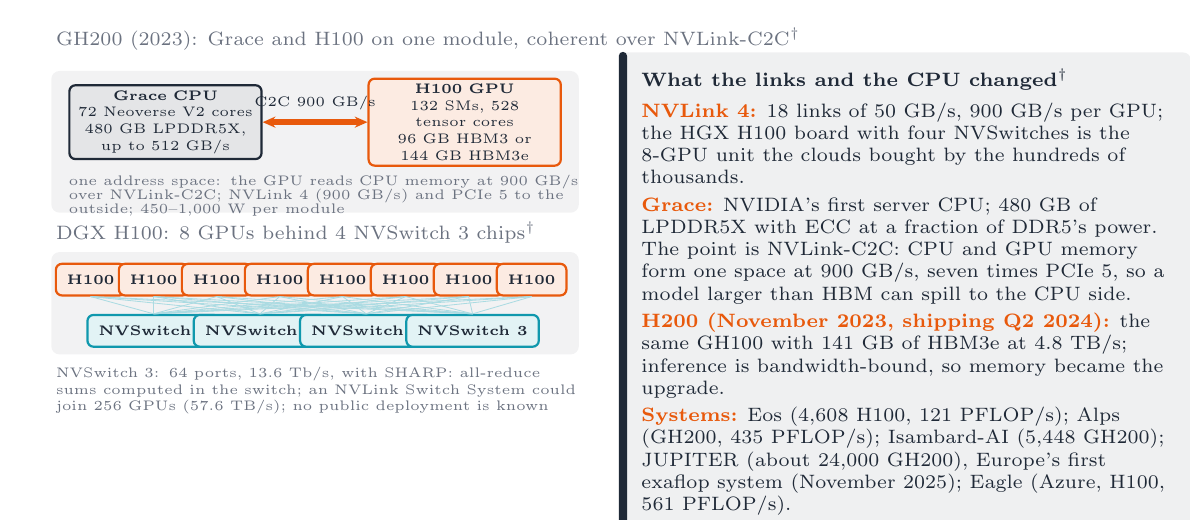
\begin{tikzpicture}
  \useasboundingbox (0,0) rectangle (14.4,5.9);
  \node[lab,anchor=south west] at (0.3,5.55) {GH200 (2023): Grace and H100 on one module, coherent over NVLink-C2C$^\dagger$};
  \begin{scope}[shift={(0.3,3.55)}]
    \fill[ink!6,rounded corners=3pt] (0,0) rectangle (6.7,1.8);
    \node[comp=ink,minimum width=2.4cm,minimum height=0.85cm,font=\fontsize{5}{6}\selectfont,text=ink,align=center,text width=2.3cm,inner sep=2pt] (gr) at (1.45,1.15) {\textbf{Grace CPU}\\72 Neoverse V2 cores\\480 GB LPDDR5X, up to 512 GB/s};
    \node[comp=attn,minimum width=2.4cm,minimum height=0.85cm,font=\fontsize{5}{6}\selectfont,text=ink,align=center,text width=2.3cm,inner sep=2pt] (hp) at (5.25,1.15) {\textbf{H100 GPU}\\132 SMs, 528 tensor cores\\96 GB HBM3 or 144 GB HBM3e};
    \draw[attn,line width=2.2pt,<->] (gr) -- node[above,font=\fontsize{4.5}{5}\selectfont,text=ink] {C2C 900 GB/s} (hp);
    \node[font=\fontsize{4.5}{5}\selectfont,text=muted,anchor=north west,text width=6.5cm] at (0.1,0.6) {one address space: the GPU reads CPU memory at 900 GB/s over NVLink-C2C; NVLink 4 (900 GB/s) and PCIe 5 to the outside; 450--1{,}000 W per module};
  \end{scope}
  \node[lab,anchor=south west] at (0.3,3.1) {DGX H100: 8 GPUs behind 4 NVSwitch 3 chips$^\dagger$};
  \begin{scope}[shift={(0.3,1.75)}]
    \fill[ink!6,rounded corners=3pt] (0,0) rectangle (6.7,1.3);
    \foreach \g in {0,...,7}{\node[comp=attn,minimum width=0.62cm,minimum height=0.36cm,font=\fontsize{4.5}{5}\selectfont\bfseries,text=ink] (h\g) at (0.5+\g*0.8,0.95) {H100};}
    \foreach \s in {0,...,3}{\node[comp=vc,minimum width=0.95cm,minimum height=0.32cm,font=\fontsize{4.5}{5}\selectfont\bfseries,text=ink] (w\s) at (1.3+\s*1.35,0.3) {NVSwitch 3};}
    \foreach \g in {0,...,7}{\foreach \s in {0,...,3}{\draw[vc!35,line width=0.3pt] (h\g.south) -- (w\s.north);}}
  \end{scope}
  \node[lab,font=\tiny,anchor=north west,text width=6.7cm] at (0.3,1.65) {NVSwitch 3: 64 ports, 13.6 Tb/s, with SHARP: all-reduce sums computed in the switch; an NVLink Switch System could join 256 GPUs (57.6 TB/s); no public deployment is known};
  \bgpanels{7.5}{5.6}{6.7cm}{What the links and the CPU changed$^\dagger$}{%
    \hl{attn}{NVLink 4:} 18 links of 50 GB/s, 900 GB/s per GPU; the
    HGX H100 board with four NVSwitches is the 8-GPU unit the clouds
    bought by the hundreds of thousands.\\[2pt]
    \hl{attn}{Grace:} NVIDIA's first server CPU; 480 GB of LPDDR5X
    with ECC at a fraction of DDR5's power. The point is NVLink-C2C:
    CPU and GPU memory form one space at 900 GB/s, seven times PCIe
    5, so a model larger than HBM can spill to the CPU side.\\[2pt]
    \hl{attn}{H200 (November 2023, shipping Q2 2024):} the same GH100
    with 141 GB of HBM3e at 4.8 TB/s; inference is bandwidth-bound,
    so memory became the upgrade.\\[2pt]
    \hl{attn}{Systems:} Eos (4{,}608 H100, 121 PFLOP/s); Alps (GH200,
    435 PFLOP/s); Isambard-AI (5{,}448 GH200); JUPITER (about
    24{,}000 GH200), Europe's first exaflop system (November 2025);
    Eagle (Azure, H100, 561 PFLOP/s).}
\end{tikzpicture}
\end{frame}

% ---------------------------------------------------------------- 15
\begin{frame}{The memory hierarchy, and the ridge that keeps moving}
\framesubtitle{Register files and L1 barely changed per SM; L2 grew 8$\times$, HBM 21$\times$; the tensor peak grew 280$\times$.}
\centering
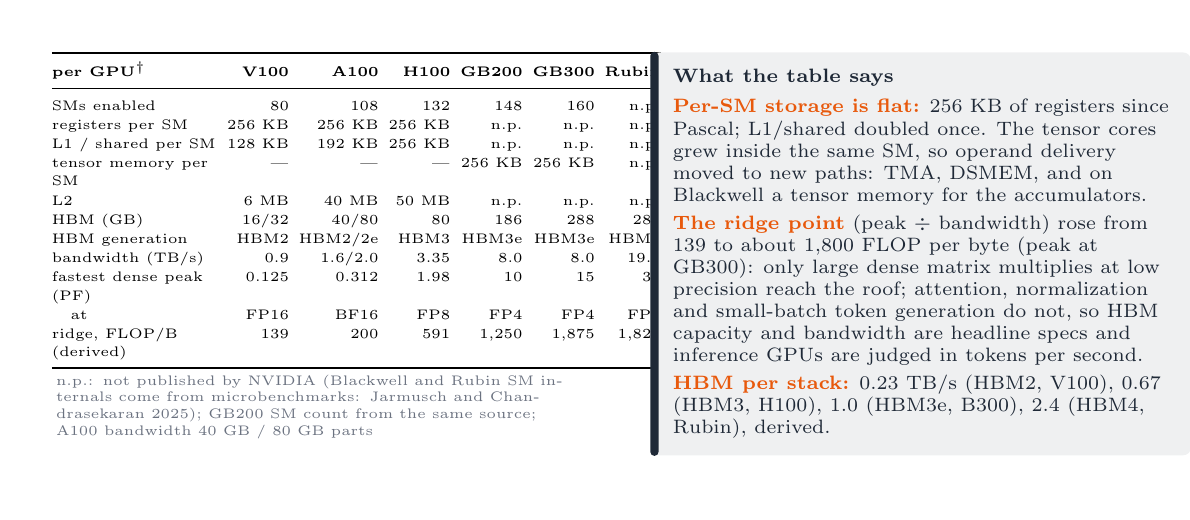
\begin{tikzpicture}
  \useasboundingbox (0,0) rectangle (14.4,5.9);
  \node[anchor=north west,inner sep=0,font=\fontsize{5.5}{6.6}\selectfont] at (0.3,5.6) {%
    \renewcommand{\arraystretch}{1.05}\setlength{\tabcolsep}{1.8pt}%
    \begin{tabular}{@{}>{\raggedright\arraybackslash}p{2.1cm}rrrrrr@{}}
      \toprule
      \textbf{per GPU}$^\dagger$ & \textbf{V100} & \textbf{A100} & \textbf{H100} & \textbf{GB200} & \textbf{GB300} & \textbf{Rubin}\\
      \midrule
      SMs enabled & 80 & 108 & 132 & 148 & 160 & n.p.\\
      registers per SM & 256 KB & 256 KB & 256 KB & n.p. & n.p. & n.p.\\
      L1 / shared per SM & 128 KB & 192 KB & 256 KB & n.p. & n.p. & n.p.\\
      tensor memory per SM & --- & --- & --- & 256 KB & 256 KB & n.p.\\
      L2 & 6 MB & 40 MB & 50 MB & n.p. & n.p. & n.p.\\
      HBM (GB) & 16/32 & 40/80 & 80 & 186 & 288 & 288\\
      HBM generation & HBM2 & HBM2/2e & HBM3 & HBM3e & HBM3e & HBM4\\
      bandwidth (TB/s) & 0.9 & 1.6/2.0 & 3.35 & 8.0 & 8.0 & 19.2\\
      fastest dense peak (PF) & 0.125 & 0.312 & 1.98 & 10 & 15 & 35\\
      \quad at & FP16 & BF16 & FP8 & FP4 & FP4 & FP4\\
      ridge, FLOP/B (derived) & 139 & 200 & 591 & 1{,}250 & 1{,}875 & 1{,}823\\
      \bottomrule
    \end{tabular}};
  \node[lab,font=\tiny,anchor=north west,text width=6.7cm] at (0.3,1.55) {n.p.: not published by NVIDIA (Blackwell and Rubin SM internals come from microbenchmarks: Jarmusch and Chandrasekaran 2025); GB200 SM count from the same source; A100 bandwidth 40 GB / 80 GB parts};
  \bgpanels{7.9}{5.6}{6.3cm}{What the table says}{%
    \hl{attn}{Per-SM storage is flat:} 256 KB of registers since
    Pascal; L1/shared doubled once. The tensor cores grew inside the
    same SM, so operand delivery moved to new paths: TMA, DSMEM, and
    on Blackwell a tensor memory for the accumulators.\\[2pt]
    \hl{attn}{The ridge point} (peak $\div$ bandwidth) rose from 139
    to about 1{,}800 FLOP per byte (peak at GB300): only large dense
    matrix multiplies at low precision reach the roof; attention,
    normalization and small-batch token generation do not, so HBM
    capacity and bandwidth are headline specs and inference GPUs are
    judged in tokens per second.\\[2pt]
    \hl{attn}{HBM per stack:} 0.23 TB/s (HBM2, V100), 0.67 (HBM3,
    H100), 1.0 (HBM3e, B300), 2.4 (HBM4, Rubin), derived.}
\end{tikzpicture}
\end{frame}

% ---------------------------------------------------------------- 16
\stage{5}
\begin{frame}{Ada Lovelace (2022): the graphics die, and the L40S}
\framesubtitle{Hopper's twin on the same process spends its area on ray tracing, a 96 MB L2 and video.}
\centering
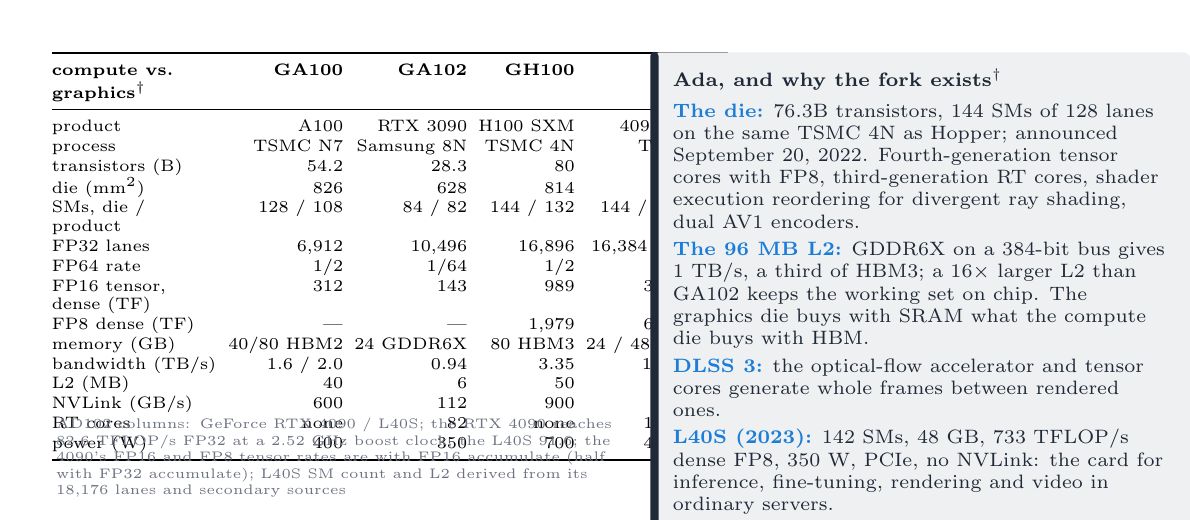
\begin{tikzpicture}
  \useasboundingbox (0,0) rectangle (14.4,5.9);
  \node[anchor=north west,inner sep=0,font=\fontsize{5.7}{6.8}\selectfont] at (0.3,5.6) {%
    \renewcommand{\arraystretch}{1.05}\setlength{\tabcolsep}{2.0pt}%
    \begin{tabular}{@{}>{\raggedright\arraybackslash}p{2.1cm}rrrr@{}}
      \toprule
      \textbf{compute vs.\ graphics}$^\dagger$ & \textbf{GA100} & \textbf{GA102} & \textbf{GH100} & \textbf{AD102}\\
      \midrule
      product & A100 & RTX 3090 & H100 SXM & 4090 / L40S\\
      process & TSMC N7 & Samsung 8N & TSMC 4N & TSMC 4N\\
      transistors (B) & 54.2 & 28.3 & 80 & 76.3\\
      die (mm$^2$) & 826 & 628 & 814 & 608\\
      SMs, die / product & 128 / 108 & 84 / 82 & 144 / 132 & 144 / 128, 142\\
      FP32 lanes & 6{,}912 & 10{,}496 & 16{,}896 & 16{,}384 / 18{,}176\\
      FP64 rate & 1/2 & 1/64 & 1/2 & 1/64\\
      FP16 tensor, dense (TF) & 312 & 143 & 989 & 330 / 362\\
      FP8 dense (TF) & --- & --- & 1{,}979 & 661 / 733\\
      memory (GB) & 40/80 HBM2 & 24 GDDR6X & 80 HBM3 & 24 / 48 GDDR6\\
      bandwidth (TB/s) & 1.6 / 2.0 & 0.94 & 3.35 & 1.0 / 0.86\\
      L2 (MB) & 40 & 6 & 50 & 72 / 96\\
      NVLink (GB/s) & 600 & 112 & 900 & none\\
      RT cores & none & 82 & none & 128 / 142\\
      power (W) & 400 & 350 & 700 & 450 / 350\\
      \bottomrule
    \end{tabular}};
  \node[lab,font=\tiny,anchor=north west,text width=7.2cm] at (0.3,1.0) {AD102 columns: GeForce RTX 4090 / L40S; the RTX 4090 reaches 82.6 TFLOP/s FP32 at a 2.52 GHz boost clock, the L40S 91.6; the 4090's FP16 and FP8 tensor rates are with FP16 accumulate (half with FP32 accumulate); L40S SM count and L2 derived from its 18{,}176 lanes and secondary sources};
  \bgpanels{7.9}{5.6}{6.3cm}{Ada, and why the fork exists$^\dagger$}{%
    \hl{mlp}{The die:} 76.3B transistors, 144 SMs of 128 lanes on the
    same TSMC 4N as Hopper; announced September 20, 2022.
    Fourth-generation tensor cores with FP8, third-generation RT
    cores, shader execution reordering for divergent ray shading,
    dual AV1 encoders.\\[2pt]
    \hl{mlp}{The 96 MB L2:} GDDR6X on a 384-bit bus gives 1 TB/s, a
    third of HBM3; a 16$\times$ larger L2 than GA102 keeps the
    working set on chip. The graphics die buys with SRAM what the
    compute die buys with HBM.\\[2pt]
    \hl{mlp}{DLSS 3:} the optical-flow accelerator and tensor cores
    generate whole frames between rendered ones.\\[2pt]
    \hl{mlp}{L40S (2023):} 142 SMs, 48 GB, 733 TFLOP/s dense FP8, 350
    W, PCIe, no NVLink: the card for inference, fine-tuning,
    rendering and video in ordinary servers.}
\end{tikzpicture}
\end{frame}

% ---------------------------------------------------------------- 17
\stage{6}
\begin{frame}{Blackwell B200 (2024): two reticle-limited dies as one GPU}
\framesubtitle{March 2024, shipping from Q4 2024: 208B transistors on TSMC 4NP, joined by a 10 TB/s die-to-die link.}
\centering
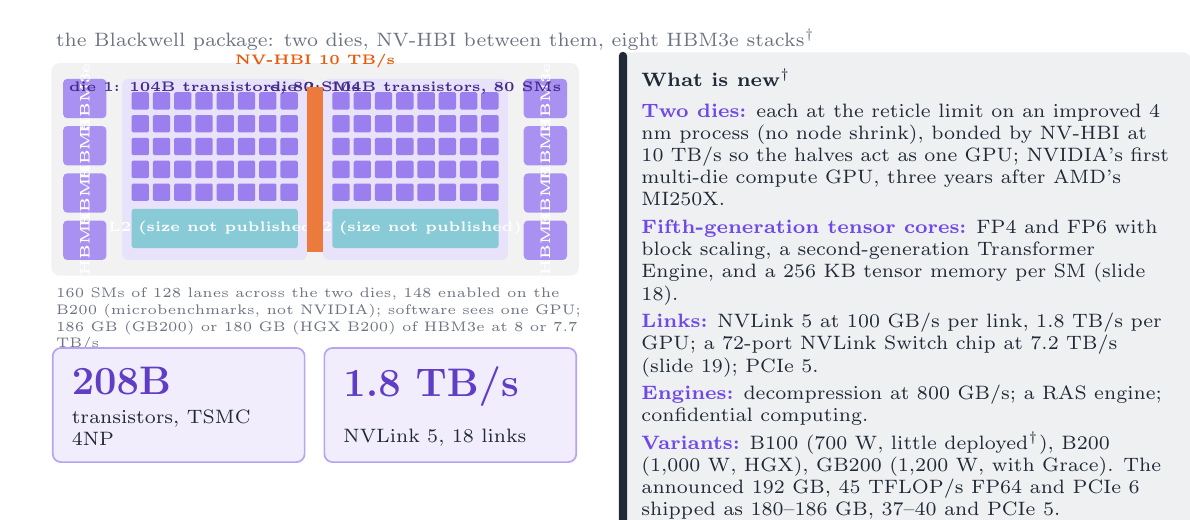
\begin{tikzpicture}
  \useasboundingbox (0,0) rectangle (14.4,5.9);
  \node[lab,anchor=south west] at (0.3,5.55) {the Blackwell package: two dies, NV-HBI between them, eight HBM3e stacks$^\dagger$};
  \begin{scope}[shift={(0.3,2.75)}]
    \fill[ink!6,rounded corners=3pt] (0,0) rectangle (6.7,2.7);
    \foreach \s in {0,...,3}{\fill[posc!60,rounded corners=1.5pt] (0.15,0.2+\s*0.6) rectangle ++(0.55,0.5); \node[font=\fontsize{4.5}{5}\selectfont\bfseries,text=white,rotate=90] at (0.425,0.45+\s*0.6) {HBM3e};
      \fill[posc!60,rounded corners=1.5pt] (6.0,0.2+\s*0.6) rectangle ++(0.55,0.5); \node[font=\fontsize{4.5}{5}\selectfont\bfseries,text=white,rotate=90] at (6.275,0.45+\s*0.6) {HBM3e};}
    \fill[posc!16,rounded corners=2pt] (0.9,0.2) rectangle (3.25,2.5); \fill[posc!16,rounded corners=2pt] (3.45,0.2) rectangle (5.8,2.5);
    \foreach \d/\x in {0/0.9,1/3.45}{\foreach \r in {0,...,4}{\foreach \c in {0,...,7}{\fill[posc!70,rounded corners=0.5pt] (\x+0.12+\c*0.27,0.95+\r*0.29) rectangle ++(0.22,0.22);}}
      \node[font=\fontsize{4.5}{5}\selectfont\bfseries,text=posc!60!black] at (\x+1.175,2.38) {die \the\numexpr\d+1\relax: 104B transistors, 80 SMs};
      \fill[vc!50,rounded corners=1pt] (\x+0.12,0.35) rectangle (\x+2.23,0.85); \node[font=\fontsize{4.5}{5}\selectfont\bfseries,text=white] at (\x+1.175,0.6) {L2 (size not published)};}
    \fill[attn!80] (3.25,0.3) rectangle (3.45,2.4); \node[font=\fontsize{4.5}{5}\selectfont\bfseries,text=attn,rotate=90] at (3.35,1.35) {};
    \node[font=\fontsize{4.5}{5}\selectfont\bfseries,text=attn,anchor=south] at (3.35,2.52) {NV-HBI 10 TB/s};
  \end{scope}
  \node[lab,font=\tiny,anchor=north west,text width=6.7cm] at (0.3,2.65) {160 SMs of 128 lanes across the two dies, 148 enabled on the B200 (microbenchmarks, not NVIDIA); software sees one GPU; 186 GB (GB200) or 180 GB (HGX B200) of HBM3e at 8 or 7.7 TB/s};
  \stat{0.3}{1.85}{208B}{transistors, TSMC 4NP}{posc}
  \stat{3.75}{1.85}{1.8 TB/s}{NVLink 5, 18 links}{posc}
  \bgpanels{7.5}{5.6}{6.7cm}{What is new$^\dagger$}{%
    \hl{posc}{Two dies:} each at the reticle limit on an improved 4
    nm process (no node shrink), bonded by NV-HBI at 10 TB/s so the
    halves act as one GPU; NVIDIA's first multi-die compute GPU,
    three years after AMD's MI250X.\\[2pt]
    \hl{posc}{Fifth-generation tensor cores:} FP4 and FP6 with
    block scaling, a second-generation Transformer Engine, and a 256
    KB tensor memory per SM (slide 18).\\[2pt]
    \hl{posc}{Links:} NVLink 5 at 100 GB/s per link, 1.8 TB/s per
    GPU; a 72-port NVLink Switch chip at 7.2 TB/s (slide 19); PCIe
    5.\\[2pt]
    \hl{posc}{Engines:} decompression at 800 GB/s; a RAS engine;
    confidential computing.\\[2pt]
    \hl{posc}{Variants:} B100 (700 W, little deployed$^\dagger$), B200 (1{,}000 W, HGX),
    GB200 (1{,}200 W, with Grace). The announced 192 GB, 45 TFLOP/s
    FP64 and PCIe 6 shipped as 180--186 GB, 37--40 and PCIe 5.}
\end{tikzpicture}
\end{frame}

% ---------------------------------------------------------------- 18
\begin{frame}{Fifth-generation tensor cores: FP4 and tensor memory}
\framesubtitle{Four-bit values with one scale per block of 16 or 32; accumulators move out of the register file.}
\centering
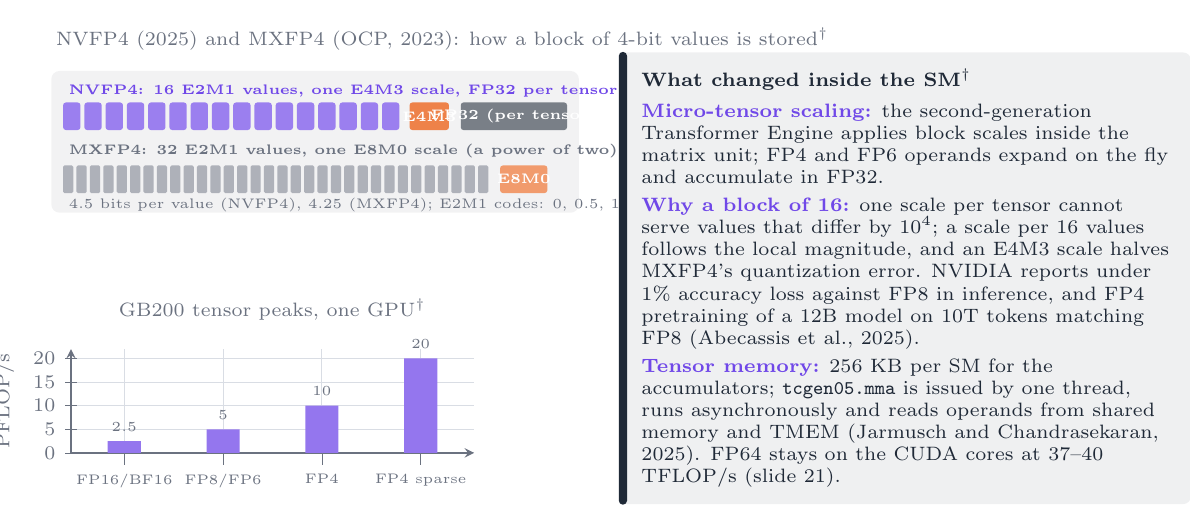
\begin{tikzpicture}
  \useasboundingbox (0,0) rectangle (14.4,5.9);
  \node[lab,anchor=south west] at (0.3,5.55) {NVFP4 (2025) and MXFP4 (OCP, 2023): how a block of 4-bit values is stored$^\dagger$};
  \begin{scope}[shift={(0.3,3.55)}]
    \fill[ink!6,rounded corners=3pt] (0,0) rectangle (6.7,1.8);
    \node[font=\tiny\bfseries,text=posc,anchor=west] at (0.1,1.55) {NVFP4: 16 E2M1 values, one E4M3 scale, FP32 per tensor};
    \foreach \i in {0,...,15}{\fill[posc!70,rounded corners=1pt] (0.15+\i*0.27,1.05) rectangle ++(0.22,0.35);}
    \fill[attn!75,rounded corners=1pt] (4.55,1.05) rectangle ++(0.5,0.35); \node[font=\fontsize{4.5}{5}\selectfont\bfseries,text=white] at (4.8,1.225) {E4M3};
    \fill[ink!60,rounded corners=1pt] (5.2,1.05) rectangle ++(1.35,0.35); \node[font=\fontsize{4.5}{5}\selectfont\bfseries,text=white] at (5.875,1.225) {FP32 (per tensor)};
    \node[font=\tiny\bfseries,text=muted,anchor=west] at (0.1,0.78) {MXFP4: 32 E2M1 values, one E8M0 scale (a power of two)};
    \foreach \i in {0,...,31}{\fill[muted!55,rounded corners=0.5pt] (0.15+\i*0.17,0.25) rectangle ++(0.13,0.35);}
    \fill[attn!60,rounded corners=1pt] (5.7,0.25) rectangle ++(0.6,0.35); \node[font=\fontsize{4.5}{5}\selectfont\bfseries,text=white] at (6.0,0.425) {E8M0};
    \node[font=\fontsize{4.5}{5}\selectfont,text=muted,anchor=west] at (0.1,0.1) {4.5 bits per value (NVFP4), 4.25 (MXFP4); E2M1 codes: 0, 0.5, 1, 1.5, 2, 3, 4, 6 and their negatives};
  \end{scope}
  \begin{scope}[shift={(0.55,0.5)}]
  \begin{axis}[lecture,width=6.7cm,height=2.9cm,ybar,bar width=12pt,ymin=0,ymax=22,enlarge x limits=0.18,
      symbolic x coords={FP16/BF16,FP8/FP6,FP4,FP4 sparse},xtick=data,xticklabel style={font=\tiny},
      ylabel={PFLOP/s},ytick={0,5,10,15,20},
      nodes near coords,nodes near coords style={font=\tiny,text=muted},point meta=rawy,
      title style={font=\scriptsize,text=muted,at={(0.5,1.02)}},title={GB200 tensor peaks, one GPU$^\dagger$}]
    \addplot[fill=posc!75,draw=none] coordinates {(FP16/BF16,2.5) (FP8/FP6,5) (FP4,10) (FP4 sparse,20)};
  \end{axis}
  \end{scope}
  \bgpanels{7.5}{5.6}{6.7cm}{What changed inside the SM$^\dagger$}{%
    \hl{posc}{Micro-tensor scaling:} the second-generation Transformer
    Engine applies block scales inside the matrix unit; FP4 and FP6
    operands expand on the fly and accumulate in FP32.\\[2pt]
    \hl{posc}{Why a block of 16:} one scale per tensor cannot serve
    values that differ by $10^4$; a scale per 16 values follows the
    local magnitude, and an E4M3 scale halves MXFP4's quantization
    error. NVIDIA reports under 1\% accuracy loss against FP8 in
    inference, and FP4 pretraining of a 12B model on 10T tokens
    matching FP8 (Abecassis et al., 2025).\\[2pt]
    \hl{posc}{Tensor memory:} 256 KB per SM for the accumulators;
    \texttt{tcgen05.mma} is issued by one thread, runs asynchronously
    and reads operands from shared memory and TMEM (Jarmusch and
    Chandrasekaran, 2025). FP64 stays on the CUDA cores at 37--40
    TFLOP/s (slide 21).}
\end{tikzpicture}
\end{frame}

% ---------------------------------------------------------------- 19
\begin{frame}{NVLink 5 and the GB200 NVL72: the rack as the unit}
\framesubtitle{72 GPUs and 36 Grace CPUs in one liquid-cooled rack; every GPU 1.8 TB/s from every other; 120 kW.}
\centering
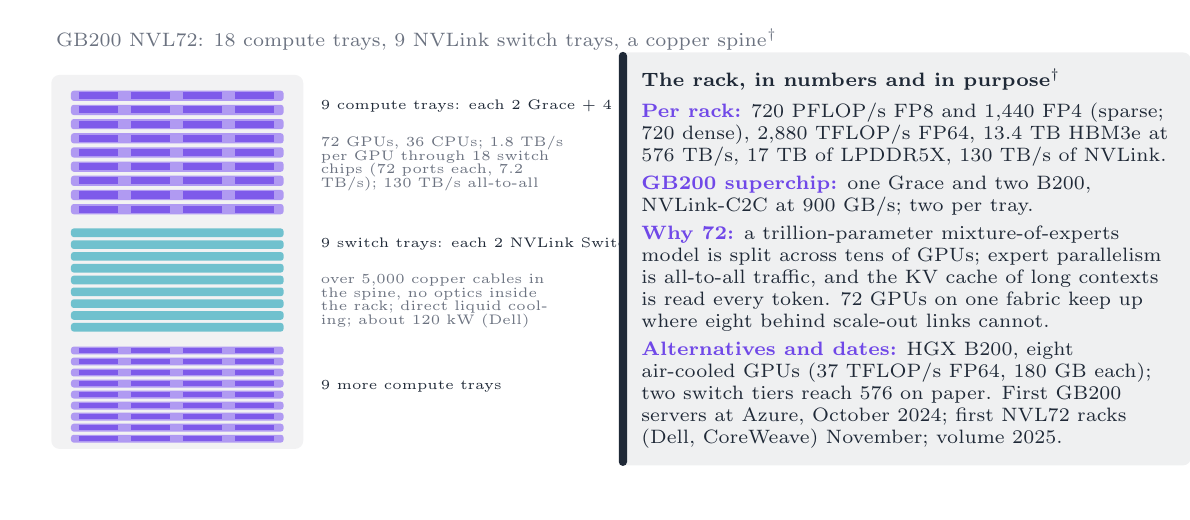
\begin{tikzpicture}
  \useasboundingbox (0,0) rectangle (14.4,5.9);
  \node[lab,anchor=south west] at (0.3,5.55) {GB200 NVL72: 18 compute trays, 9 NVLink switch trays, a copper spine$^\dagger$};
  \begin{scope}[shift={(0.3,0.55)}]
    \fill[ink!6,rounded corners=3pt] (0,0) rectangle (3.2,4.75);
    \foreach \t in {0,...,8}{\fill[posc!55,rounded corners=1pt] (0.25,4.42-\t*0.18) rectangle (2.95,4.55-\t*0.18);
      \foreach \g in {0,...,3}{\fill[posc!90] (0.35+\g*0.66,4.44-\t*0.18) rectangle ++(0.5,0.09);}}
    \foreach \t in {0,...,8}{\fill[vc!60,rounded corners=1pt] (0.25,2.69-\t*0.15) rectangle (2.95,2.8-\t*0.15);}
    \foreach \t in {0,...,8}{\fill[posc!55,rounded corners=1pt] (0.25,1.2-\t*0.14) rectangle (2.95,1.3-\t*0.14);
      \foreach \g in {0,...,3}{\fill[posc!90] (0.35+\g*0.66,1.215-\t*0.14) rectangle ++(0.5,0.07);}}
    \node[font=\fontsize{4.5}{5}\selectfont,text=ink,anchor=west] at (3.3,4.35) {9 compute trays: each 2 Grace $+$ 4 B200};
    \node[font=\fontsize{4.5}{5}\selectfont,text=muted,anchor=north west,text width=3.3cm] at (3.3,4.1) {72 GPUs, 36 CPUs; 1.8 TB/s per GPU through 18 switch chips (72 ports each, 7.2 TB/s); 130 TB/s all-to-all};
    \node[font=\fontsize{4.5}{5}\selectfont,text=ink,anchor=west] at (3.3,2.6) {9 switch trays: each 2 NVLink Switch chips};
    \node[font=\fontsize{4.5}{5}\selectfont,text=muted,anchor=north west,text width=3.3cm] at (3.3,2.35) {over 5{,}000 copper cables in the spine, no optics inside the rack; direct liquid cooling; about 120 kW (Dell)};
    \node[font=\fontsize{4.5}{5}\selectfont,text=ink,anchor=west] at (3.3,0.8) {9 more compute trays};
  \end{scope}
  \bgpanels{7.5}{5.6}{6.7cm}{The rack, in numbers and in purpose$^\dagger$}{%
    \hl{posc}{Per rack:} 720 PFLOP/s FP8 and 1{,}440 FP4 (sparse; 720
    dense), 2{,}880 TFLOP/s FP64, 13.4 TB HBM3e at 576 TB/s, 17 TB of
    LPDDR5X, 130 TB/s of NVLink.\\[2pt]
    \hl{posc}{GB200 superchip:} one Grace and two B200, NVLink-C2C
    at 900 GB/s; two per tray.\\[2pt]
    \hl{posc}{Why 72:} a trillion-parameter mixture-of-experts model
    is split across tens of GPUs; expert parallelism is all-to-all
    traffic, and the KV cache of long contexts is read every token.
    72 GPUs on one fabric keep up where eight behind scale-out links
    cannot.\\[2pt]
    \hl{posc}{Alternatives and dates:} HGX B200, eight air-cooled GPUs
    (37 TFLOP/s FP64, 180 GB each); two switch tiers reach 576 on
    paper. First GB200 servers at Azure, October 2024; first NVL72
    racks (Dell, CoreWeave) November; volume 2025.}
\end{tikzpicture}
\end{frame}

% ---------------------------------------------------------------- 20
\begin{frame}{Blackwell Ultra (2025): more HBM, 1.5$\times$ FP4, almost no FP64}
\framesubtitle{Same dies, re-balanced: 288 GB of HBM3e, 1.5$\times$ FP4, 2$\times$ exponentials, FP64 cut to 1.4 TFLOP/s.}
\centering
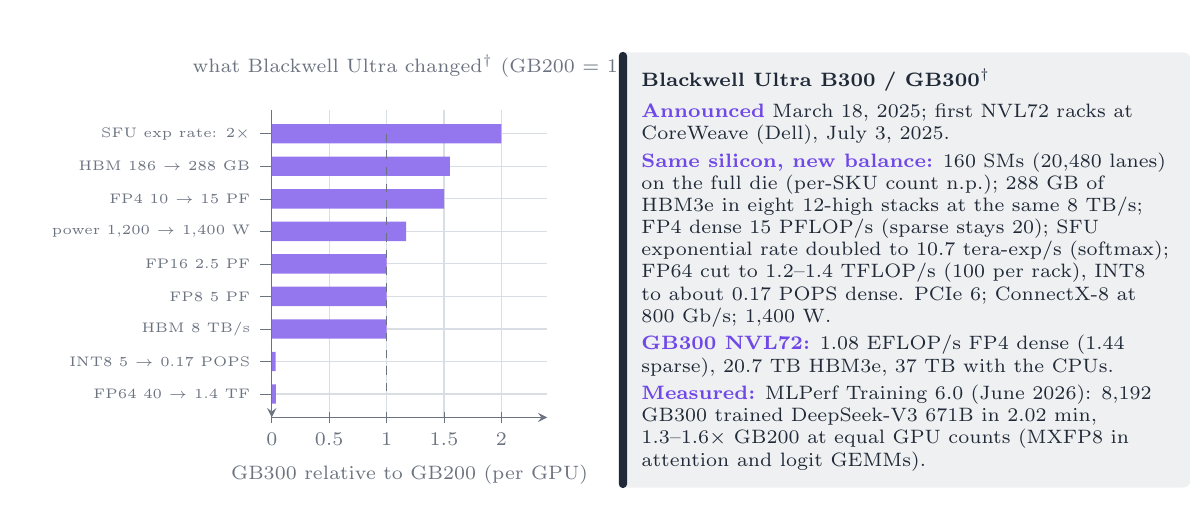
\begin{tikzpicture}
  \useasboundingbox (0,0) rectangle (14.4,5.9);
  \begin{scope}[shift={(3.1,0.95)}]
  \begin{axis}[lecture,scale only axis,width=3.5cm,height=3.9cm,xbar,bar width=7pt,xmin=0,xmax=2.4,enlarge y limits=0.09,
      symbolic y coords={{SFU exp rate: 2$\times$},{HBM 186 $\to$ 288 GB},{FP4 10 $\to$ 15 PF},{power 1{,}200 $\to$ 1{,}400 W},{FP16 2.5 PF},{FP8 5 PF},{HBM 8 TB/s},{INT8 5 $\to$ 0.17 POPS},{FP64 40 $\to$ 1.4 TF}},
      ytick=data,y dir=reverse,yticklabel style={font=\tiny},xlabel={GB300 relative to GB200 (per GPU)},
      xtick={0,0.5,1,1.5,2},
      title style={font=\scriptsize,text=muted,at={(0.5,1.02)}},title={what Blackwell Ultra changed$^\dagger$ (GB200 $=$ 1)}]
    \addplot[fill=posc!75,draw=none] coordinates {(2,{SFU exp rate: 2$\times$}) (1.55,{HBM 186 $\to$ 288 GB}) (1.5,{FP4 10 $\to$ 15 PF}) (1.17,{power 1{,}200 $\to$ 1{,}400 W}) (1,{FP16 2.5 PF}) (1,{FP8 5 PF}) (1,{HBM 8 TB/s}) (0.034,{INT8 5 $\to$ 0.17 POPS}) (0.035,{FP64 40 $\to$ 1.4 TF})};
    \draw[muted,dashed] (axis cs:1,{SFU exp rate: 2$\times$}) -- (axis cs:1,{FP64 40 $\to$ 1.4 TF});
  \end{axis}
  \end{scope}
  \bgpanels{7.5}{5.6}{6.7cm}{Blackwell Ultra B300 / GB300$^\dagger$}{%
    \hl{posc}{Announced} March 18, 2025; first NVL72 racks at
    CoreWeave (Dell), July 3, 2025.\\[2pt]
    \hl{posc}{Same silicon, new balance:} 160 SMs (20{,}480 lanes) on
    the full die (per-SKU count n.p.); 288 GB of HBM3e in
    eight 12-high stacks at the same 8 TB/s; FP4 dense 15 PFLOP/s
    (sparse stays 20); SFU exponential rate doubled to 10.7
    tera-exp/s (softmax); FP64 cut to 1.2--1.4 TFLOP/s (100 per
    rack), INT8 to about 0.17 POPS dense. PCIe 6; ConnectX-8 at 800
    Gb/s; 1{,}400 W.\\[2pt]
    \hl{posc}{GB300 NVL72:} 1.08 EFLOP/s FP4 dense (1.44 sparse),
    20.7 TB HBM3e, 37 TB with the CPUs.\\[2pt]
    \hl{posc}{Measured:} MLPerf Training 6.0 (June 2026): 8{,}192
    GB300 trained DeepSeek-V3 671B in 2.02 min, 1.3--1.6$\times$ GB200
    at equal GPU counts (MXFP8 in attention and logit GEMMs).}
\end{tikzpicture}
\end{frame}

% ---------------------------------------------------------------- 21
\begin{frame}{FP64: what happened to double precision}
\framesubtitle{Up nearly 9$\times$ to H100, flat on Blackwell, nearly gone on Blackwell Ultra, back to 33 TFLOP/s on Rubin.}
\centering
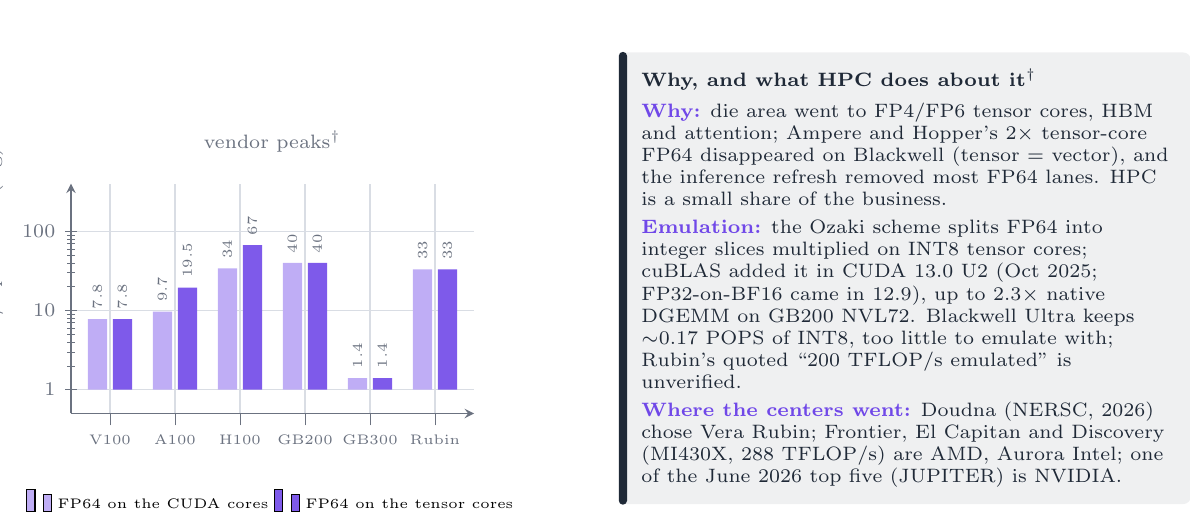
\begin{tikzpicture}
  \useasboundingbox (0,0) rectangle (14.4,5.9);
  \begin{scope}[shift={(0.55,1.0)}]
  \begin{axis}[lecture,width=6.7cm,height=4.5cm,ybar,bar width=7pt,ymode=log,ymin=0.5,ymax=400,enlarge x limits=0.12,
      symbolic x coords={V100,A100,H100,GB200,GB300,Rubin},xtick=data,xticklabel style={font=\tiny},
      ylabel={FP64 TFLOP/s per GPU (log)},ytick={1,10,100},yticklabels={1,10,100},
      nodes near coords,nodes near coords style={font=\tiny,text=muted,rotate=90,anchor=west},point meta=rawy,
      legend style={at={(0.5,-0.3)},anchor=north,font=\tiny,legend columns=2},
      title style={font=\scriptsize,text=muted,at={(0.5,1.02)}},title={vendor peaks$^\dagger$}]
    \addplot[fill=posc!45,draw=none] coordinates {(V100,7.8) (A100,9.7) (H100,34) (GB200,40) (GB300,1.4) (Rubin,33)};
    \addlegendentry{FP64 on the CUDA cores}
    \addplot[fill=posc!90,draw=none] coordinates {(V100,7.8) (A100,19.5) (H100,67) (GB200,40) (GB300,1.4) (Rubin,33)};
    \addlegendentry{FP64 on the tensor cores}
  \end{axis}
  \end{scope}
  \bgpanels{7.5}{5.6}{6.7cm}{Why, and what HPC does about it$^\dagger$}{%
    \hl{posc}{Why:} die area went to FP4/FP6 tensor cores, HBM and
    attention; Ampere and Hopper's 2$\times$ tensor-core FP64
    disappeared on Blackwell (tensor $=$ vector), and the inference
    refresh removed most FP64 lanes. HPC is a small share of the
    business.\\[2pt]
    \hl{posc}{Emulation:} the Ozaki scheme splits FP64 into integer
    slices multiplied on INT8 tensor cores; cuBLAS added it in CUDA
    13.0 U2 (Oct 2025; FP32-on-BF16 came in 12.9), up to 2.3$\times$
    native DGEMM on GB200 NVL72. Blackwell Ultra keeps ${\sim}$0.17
    POPS of INT8, too little to emulate with; Rubin's quoted ``200
    TFLOP/s emulated'' is unverified.\\[2pt]
    \hl{posc}{Where the centers went:} Doudna (NERSC, 2026) chose Vera
    Rubin; Frontier, El Capitan and Discovery (MI430X, 288 TFLOP/s)
    are AMD, Aurora Intel; one of the June 2026 top five (JUPITER) is
    NVIDIA.}
\end{tikzpicture}
\end{frame}

% ---------------------------------------------------------------- 22
\begin{frame}{Power: 300 W to 1,400 W per GPU, 120 kW to 600 kW per rack}
\framesubtitle{Perf per watt rose mostly by cutting precision; the rest was bought with power and liquid cooling.}
\centering
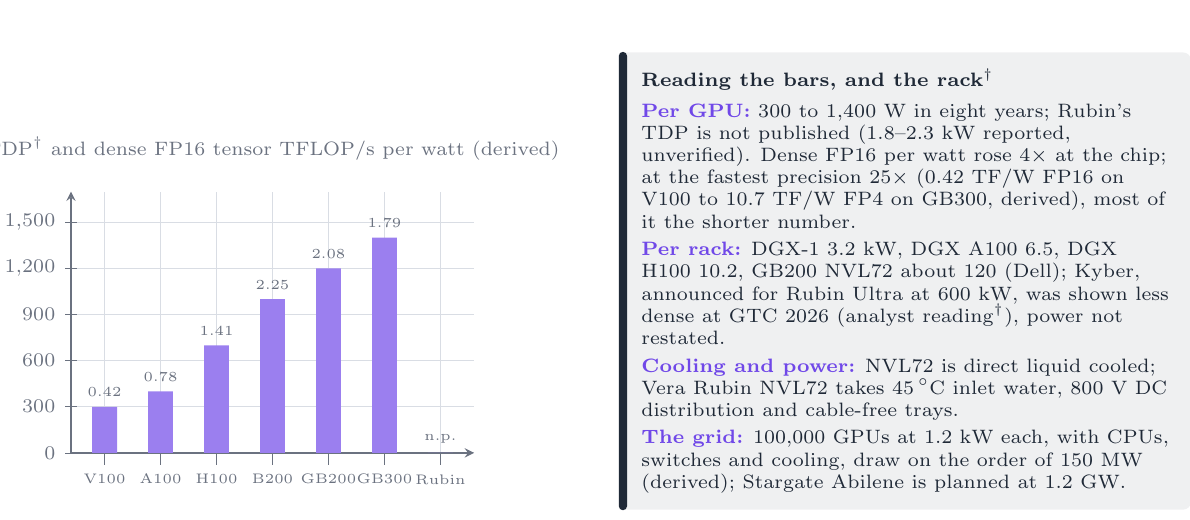
\begin{tikzpicture}
  \useasboundingbox (0,0) rectangle (14.4,5.9);
  \begin{scope}[shift={(0.55,0.5)}]
  \begin{axis}[lecture,width=6.7cm,height=4.9cm,ybar,bar width=9pt,ymin=0,ymax=1700,enlarge x limits=0.1,
      symbolic x coords={V100,A100,H100,B200,GB200,GB300,Rubin},xtick=data,xticklabel style={font=\tiny},
      ylabel={GPU power (W)},ytick={0,300,600,900,1200,1500},
      nodes near coords,nodes near coords style={font=\tiny,text=muted},point meta=explicit symbolic,
      title style={font=\scriptsize,text=muted,at={(0.5,1.02)}},title={TDP$^\dagger$ and dense FP16 tensor TFLOP/s per watt (derived)}]
    \addplot[fill=posc!70,draw=none] coordinates {(V100,300)[0.42] (A100,400)[0.78] (H100,700)[1.41] (B200,1000)[2.25] (GB200,1200)[2.08] (GB300,1400)[1.79] (Rubin,0)[n.p.]};
  \end{axis}
  \end{scope}
  \bgpanels{7.5}{5.6}{6.7cm}{Reading the bars, and the rack$^\dagger$}{%
    \hl{posc}{Per GPU:} 300 to 1{,}400 W in eight years; Rubin's TDP
    is not published (1.8--2.3 kW reported, unverified). Dense FP16
    per watt rose 4$\times$ at the chip; at the fastest precision
    25$\times$ (0.42 TF/W FP16 on V100 to 10.7 TF/W FP4 on GB300,
    derived), most of it the shorter number.\\[2pt]
    \hl{posc}{Per rack:} DGX-1 3.2 kW, DGX A100 6.5, DGX H100 10.2,
    GB200 NVL72 about 120 (Dell); Kyber, announced for Rubin Ultra at
    600 kW, was shown less dense at GTC 2026 (analyst reading$^\dagger$),
    power not restated.\\[2pt]
    \hl{posc}{Cooling and power:} NVL72 is direct liquid cooled; Vera
    Rubin NVL72 takes 45\,$^\circ$C inlet water, 800 V DC
    distribution and cable-free trays.\\[2pt]
    \hl{posc}{The grid:} 100{,}000 GPUs at 1.2 kW each, with CPUs,
    switches and cooling, draw on the order of 150 MW (derived);
    Stargate Abilene is planned at 1.2 GW.}
\end{tikzpicture}
\end{frame}

% ---------------------------------------------------------------- 23
\stage{7}
\begin{frame}{Rubin (2026): HBM4, 3 nm, and the third dual-die GPU}
\framesubtitle{GTC 2025 specs, CES 2026 production, first racks August 2026, spec sheet revised in September 2026.}
\centering
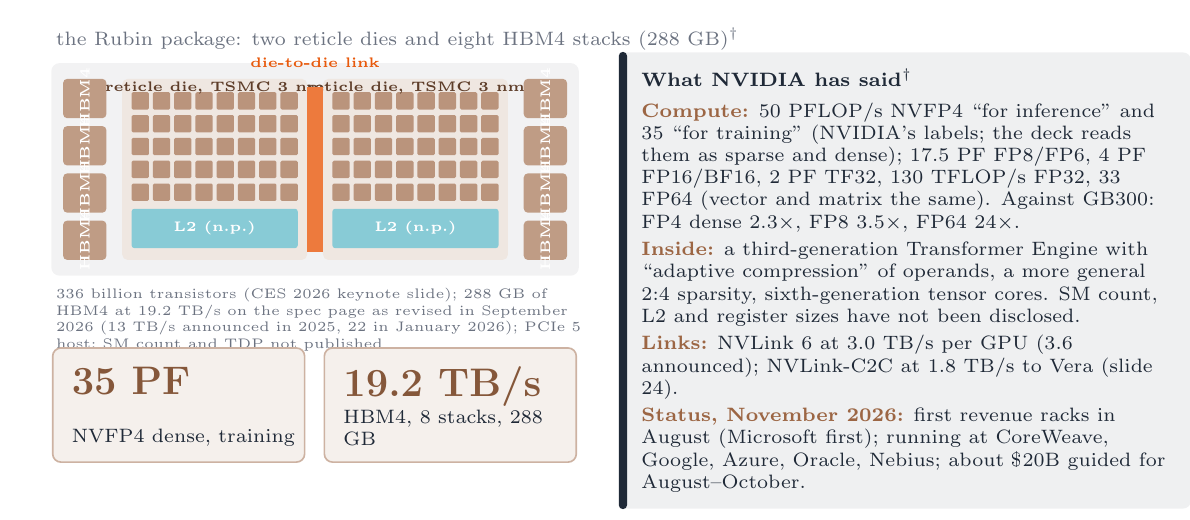
\begin{tikzpicture}
  \useasboundingbox (0,0) rectangle (14.4,5.9);
  \node[lab,anchor=south west] at (0.3,5.55) {the Rubin package: two reticle dies and eight HBM4 stacks (288 GB)$^\dagger$};
  \begin{scope}[shift={(0.3,2.75)}]
    \fill[ink!6,rounded corners=3pt] (0,0) rectangle (6.7,2.7);
    \foreach \s in {0,...,3}{\fill[trn!65,rounded corners=1.5pt] (0.15,0.2+\s*0.6) rectangle ++(0.55,0.5); \node[font=\fontsize{4.5}{5}\selectfont\bfseries,text=white,rotate=90] at (0.425,0.45+\s*0.6) {HBM4};
      \fill[trn!65,rounded corners=1.5pt] (6.0,0.2+\s*0.6) rectangle ++(0.55,0.5); \node[font=\fontsize{4.5}{5}\selectfont\bfseries,text=white,rotate=90] at (6.275,0.45+\s*0.6) {HBM4};}
    \fill[trn!16,rounded corners=2pt] (0.9,0.2) rectangle (3.25,2.5); \fill[trn!16,rounded corners=2pt] (3.45,0.2) rectangle (5.8,2.5);
    \foreach \x in {0.9,3.45}{\foreach \r in {0,...,4}{\foreach \c in {0,...,7}{\fill[trn!70,rounded corners=0.5pt] (\x+0.12+\c*0.27,0.95+\r*0.29) rectangle ++(0.22,0.22);}}
      \node[font=\fontsize{4.5}{5}\selectfont\bfseries,text=trn!60!black] at (\x+1.175,2.38) {reticle die, TSMC 3 nm};
      \fill[vc!50,rounded corners=1pt] (\x+0.12,0.35) rectangle (\x+2.23,0.85); \node[font=\fontsize{4.5}{5}\selectfont\bfseries,text=white] at (\x+1.175,0.6) {L2 (n.p.)};}
    \fill[attn!80] (3.25,0.3) rectangle (3.45,2.4);
    \node[font=\fontsize{4.5}{5}\selectfont\bfseries,text=attn,anchor=south] at (3.35,2.52) {die-to-die link};
  \end{scope}
  \node[lab,font=\tiny,anchor=north west,text width=6.7cm] at (0.3,2.65) {336 billion transistors (CES 2026 keynote slide); 288 GB of HBM4 at 19.2 TB/s on the spec page as revised in September 2026 (13 TB/s announced in 2025, 22 in January 2026); PCIe 5 host; SM count and TDP not published};
  \stat{0.3}{1.85}{35 PF}{NVFP4 dense, training}{trn}
  \stat{3.75}{1.85}{19.2 TB/s}{HBM4, 8 stacks, 288 GB}{trn}
  \bgpanels{7.5}{5.6}{6.7cm}{What NVIDIA has said$^\dagger$}{%
    \hl{trn}{Compute:} 50 PFLOP/s NVFP4 ``for inference'' and 35
    ``for training'' (NVIDIA's labels; the deck reads them as sparse
    and dense); 17.5 PF FP8/FP6, 4 PF FP16/BF16, 2 PF TF32,
    130 TFLOP/s FP32, 33 FP64 (vector and matrix the same). Against
    GB300: FP4 dense 2.3$\times$, FP8 3.5$\times$, FP64 24$\times$.\\[2pt]
    \hl{trn}{Inside:} a third-generation Transformer Engine with
    ``adaptive compression'' of operands, a more general 2:4
    sparsity, sixth-generation tensor cores. SM count, L2 and
    register sizes have not been disclosed.\\[2pt]
    \hl{trn}{Links:} NVLink 6 at 3.0 TB/s per GPU (3.6 announced);
    NVLink-C2C at 1.8 TB/s to Vera (slide 24).\\[2pt]
    \hl{trn}{Status, November 2026:} first revenue racks in August
    (Microsoft first); running at CoreWeave, Google, Azure, Oracle,
    Nebius; about \$20B guided for August--October.}
\end{tikzpicture}
\end{frame}

% ---------------------------------------------------------------- 24
\begin{frame}{Vera, and the platform of six chips}
\framesubtitle{A CPU built for the rack: 88 custom cores, 1.8 TB/s to the GPUs; the generation ships as six chips.}
\centering
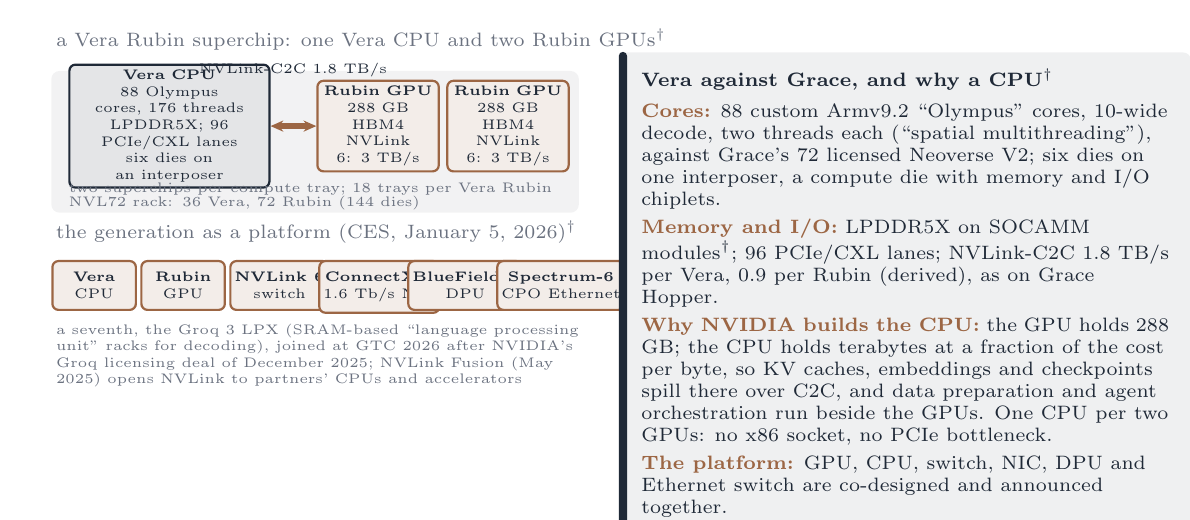
\begin{tikzpicture}
  \useasboundingbox (0,0) rectangle (14.4,5.9);
  \node[lab,anchor=south west] at (0.3,5.55) {a Vera Rubin superchip: one Vera CPU and two Rubin GPUs$^\dagger$};
  \begin{scope}[shift={(0.3,3.55)}]
    \fill[ink!6,rounded corners=3pt] (0,0) rectangle (6.7,1.8);
    \node[comp=ink,minimum width=2.5cm,minimum height=0.95cm,font=\fontsize{5}{6}\selectfont,text=ink,align=center,text width=2.4cm,inner sep=2pt] (ve) at (1.5,1.1) {\textbf{Vera CPU}\\88 Olympus cores, 176 threads\\LPDDR5X; 96 PCIe/CXL lanes\\six dies on an interposer};
    \node[comp=trn,minimum width=1.5cm,minimum height=0.95cm,font=\fontsize{5}{6}\selectfont,text=ink,align=center,text width=1.4cm,inner sep=2pt] (r1) at (4.15,1.1) {\textbf{Rubin GPU}\\288 GB HBM4\\NVLink 6: 3 TB/s};
    \node[comp=trn,minimum width=1.5cm,minimum height=0.95cm,font=\fontsize{5}{6}\selectfont,text=ink,align=center,text width=1.4cm,inner sep=2pt] (r2) at (5.8,1.1) {\textbf{Rubin GPU}\\288 GB HBM4\\NVLink 6: 3 TB/s};
    \draw[trn,line width=2pt,<->] (ve) -- (r1);
    \node[font=\fontsize{4.5}{5}\selectfont,text=ink,anchor=south] at (3.07,1.6) {NVLink-C2C 1.8 TB/s};
    \node[font=\fontsize{4.5}{5}\selectfont,text=muted,anchor=north west,text width=6.5cm] at (0.1,0.5) {two superchips per compute tray; 18 trays per Vera Rubin NVL72 rack: 36 Vera, 72 Rubin (144 dies)};
  \end{scope}
  \node[lab,anchor=south west] at (0.3,3.1) {the generation as a platform (CES, January 5, 2026)$^\dagger$};
  \foreach \i/\name/\sub in {0/Vera/{CPU},1/Rubin/{GPU},2/NVLink 6/{switch},3/ConnectX-9/{1.6 Tb/s NIC},4/BlueField-4/{DPU},5/Spectrum-6/{CPO Ethernet}}{
    \node[comp=trn,minimum width=1.06cm,minimum height=0.62cm,font=\fontsize{5}{6}\selectfont,text=ink,align=center,anchor=north west,inner xsep=1.5pt] at (0.3+\i*1.13,2.95) {\textbf{\name}\\\sub};}
  \node[lab,font=\tiny,anchor=north west,text width=6.7cm] at (0.3,2.2) {a seventh, the Groq 3 LPX (SRAM-based ``language processing unit'' racks for decoding), joined at GTC 2026 after NVIDIA's Groq licensing deal of December 2025; NVLink Fusion (May 2025) opens NVLink to partners' CPUs and accelerators};
  \bgpanels{7.5}{5.6}{6.7cm}{Vera against Grace, and why a CPU$^\dagger$}{%
    \hl{trn}{Cores:} 88 custom Armv9.2 ``Olympus'' cores, 10-wide
    decode, two threads each (``spatial multithreading''), against
    Grace's 72 licensed Neoverse V2; six dies on one interposer, a
    compute die with memory and I/O chiplets.\\[2pt]
    \hl{trn}{Memory and I/O:} LPDDR5X on SOCAMM modules$^\dagger$; 96
    PCIe/CXL lanes; NVLink-C2C 1.8 TB/s per Vera, 0.9 per Rubin
    (derived), as on Grace Hopper.\\[2pt]
    \hl{trn}{Why NVIDIA builds the CPU:} the GPU holds 288 GB; the CPU
    holds terabytes at a fraction of the cost per byte, so KV caches,
    embeddings and checkpoints spill there over C2C, and data
    preparation and agent orchestration run beside the GPUs. One CPU
    per two GPUs: no x86 socket, no PCIe bottleneck.\\[2pt]
    \hl{trn}{The platform:} GPU, CPU, switch, NIC, DPU and Ethernet
    switch are co-designed and announced together.}
\end{tikzpicture}
\end{frame}

% ---------------------------------------------------------------- 25
\begin{frame}{Vera Rubin NVL72 against the Blackwell racks}
\framesubtitle{Same 72-GPU shape; against GB200: 3.5$\times$ the dense FP4, 2.4$\times$ the HBM bandwidth, 1.7$\times$ the NVLink.}
\centering
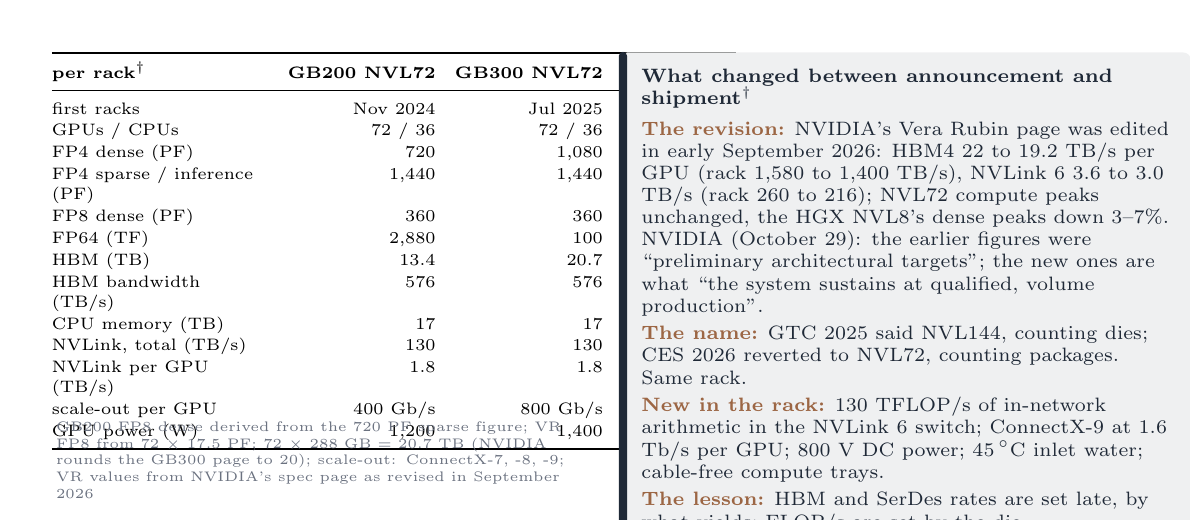
\begin{tikzpicture}
  \useasboundingbox (0,0) rectangle (14.4,5.9);
  \node[anchor=north west,inner sep=0,font=\fontsize{6.2}{7.3}\selectfont] at (0.3,5.6) {%
    \renewcommand{\arraystretch}{1.08}\setlength{\tabcolsep}{3.5pt}%
    \begin{tabular}{@{}>{\raggedright\arraybackslash}p{2.75cm}rrr@{}}
      \toprule
      \textbf{per rack}$^\dagger$ & \textbf{GB200 NVL72} & \textbf{GB300 NVL72} & \textbf{VR NVL72}\\
      \midrule
      first racks & Nov 2024 & Jul 2025 & Aug 2026\\
      GPUs / CPUs & 72 / 36 & 72 / 36 & 72 / 36\\
      FP4 dense (PF) & 720 & 1{,}080 & 2{,}520\\
      FP4 sparse / inference (PF) & 1{,}440 & 1{,}440 & 3{,}600\\
      FP8 dense (PF) & 360 & 360 & 1{,}260\\
      FP64 (TF) & 2{,}880 & 100 & 2{,}400\\
      HBM (TB) & 13.4 & 20.7 & 20.7\\
      HBM bandwidth (TB/s) & 576 & 576 & 1{,}400\\
      CPU memory (TB) & 17 & 17 & 54\\
      NVLink, total (TB/s) & 130 & 130 & 216\\
      NVLink per GPU (TB/s) & 1.8 & 1.8 & 3.0\\
      scale-out per GPU & 400 Gb/s & 800 Gb/s & 1.6 Tb/s\\
      GPU power (W) & 1{,}200 & 1{,}400 & n.p.\\
      \bottomrule
    \end{tabular}};
  \node[lab,font=\tiny,anchor=north west,text width=6.7cm] at (0.3,0.95) {GB200 FP8 dense derived from the 720 PF sparse figure; VR FP8 from 72 $\times$ 17.5 PF; 72 $\times$ 288 GB $=$ 20.7 TB (NVIDIA rounds the GB300 page to 20); scale-out: ConnectX-7, -8, -9; VR values from NVIDIA's spec page as revised in September 2026};
  \bgpanels{7.5}{5.6}{6.7cm}{What changed between announcement and shipment$^\dagger$}{%
    \hl{trn}{The revision:} NVIDIA's Vera Rubin page was edited in
    early September 2026: HBM4 22 to 19.2 TB/s per GPU (rack 1{,}580
    to 1{,}400 TB/s), NVLink 6 3.6 to 3.0 TB/s (rack 260 to 216);
    NVL72 compute peaks unchanged, the HGX NVL8's dense peaks down
    3--7\%. NVIDIA (October 29): the earlier figures
    were ``preliminary architectural targets''; the new ones are what
    ``the system sustains at qualified, volume production''.\\[2pt]
    \hl{trn}{The name:} GTC 2025 said NVL144, counting dies; CES 2026
    reverted to NVL72, counting packages. Same rack.\\[2pt]
    \hl{trn}{New in the rack:} 130 TFLOP/s of in-network arithmetic
    in the NVLink 6 switch; ConnectX-9 at 1.6 Tb/s per GPU; 800 V DC
    power; 45\,$^\circ$C inlet water; cable-free compute trays.\\[2pt]
    \hl{trn}{The lesson:} HBM and SerDes rates are set late, by what
    yields; FLOP/s are set by the die.}
\end{tikzpicture}
\end{frame}

% ---------------------------------------------------------------- 26
\begin{frame}{After Rubin: CPX, Rubin Ultra, Feynman}
\framesubtitle{Announced for 2026--28: one product dropped, one redesigned, one replaced by a licensed design.}
\centering
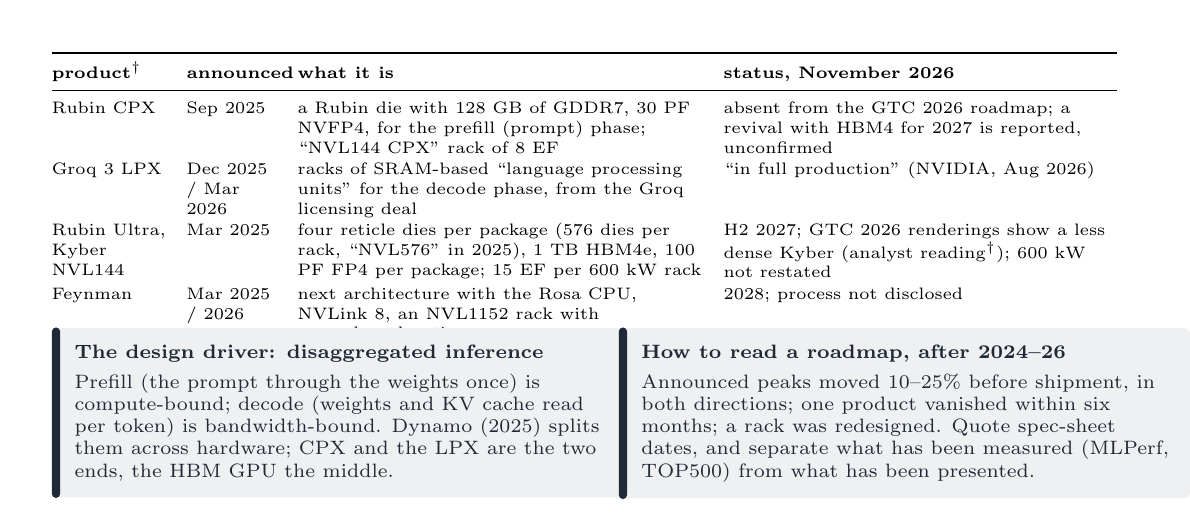
\begin{tikzpicture}
  \useasboundingbox (0,0) rectangle (14.4,5.9);
  \node[anchor=north west,inner sep=0,font=\fontsize{6.0}{7.1}\selectfont] at (0.3,5.6) {%
    \renewcommand{\arraystretch}{1.1}\setlength{\tabcolsep}{3.0pt}%
    \begin{tabular}{@{}>{\raggedright\arraybackslash}p{1.5cm}>{\raggedright\arraybackslash}p{1.2cm}>{\raggedright\arraybackslash}p{5.2cm}>{\raggedright\arraybackslash}p{5.0cm}@{}}
      \toprule
      \textbf{product}$^\dagger$ & \textbf{announced} & \textbf{what it is} & \textbf{status, November 2026}\\
      \midrule
      Rubin CPX & Sep 2025 & a Rubin die with 128 GB of GDDR7, 30 PF NVFP4, for the prefill (prompt) phase; ``NVL144 CPX'' rack of 8 EF & absent from the GTC 2026 roadmap; a revival with HBM4 for 2027 is reported, unconfirmed\\
      Groq 3 LPX & Dec 2025 / Mar 2026 & racks of SRAM-based ``language processing units'' for the decode phase, from the Groq licensing deal & ``in full production'' (NVIDIA, Aug 2026)\\
      Rubin Ultra, Kyber NVL144 & Mar 2025 & four reticle dies per package (576 dies per rack, ``NVL576'' in 2025), 1 TB HBM4e, 100 PF FP4 per package; 15 EF per 600 kW rack & H2 2027; GTC 2026 renderings show a less dense Kyber (analyst reading$^\dagger$); 600 kW not restated\\
      Feynman & Mar 2025 / 2026 & next architecture with the Rosa CPU, NVLink 8, an NVL1152 rack with co-packaged optics & 2028; process not disclosed\\
      NVLink Fusion & May 2025 & NVLink IP for partners' CPUs and accelerators (MediaTek, Marvell, Qualcomm, Fujitsu, Intel) & design-ins announced, no shipping product cited\\
      \bottomrule
    \end{tabular}};
  \bgpanels{0.3}{2.1}{6.7cm}{The design driver: disaggregated inference}{%
    Prefill (the prompt through the weights once) is compute-bound;
    decode (weights and KV cache read per token) is bandwidth-bound.
    Dynamo (2025) splits them across hardware; CPX and the LPX are
    the two ends, the HBM GPU the middle.}
  \bgpanels{7.5}{2.1}{6.7cm}{How to read a roadmap, after 2024--26}{%
    Announced peaks moved 10--25\% before shipment, in both
    directions; one product vanished within six months; a rack was
    redesigned. Quote spec-sheet dates, and separate what has been
    measured (MLPerf, TOP500) from what has been presented.}
\end{tikzpicture}
\end{frame}

% ---------------------------------------------------------------- 27
\stage{8}
\begin{frame}{Where they run: NVIDIA systems, 2020--2026}
\framesubtitle{Centers bought A100, H100 and GH200 machines; the largest Blackwell installations do not run HPL.}
\centering
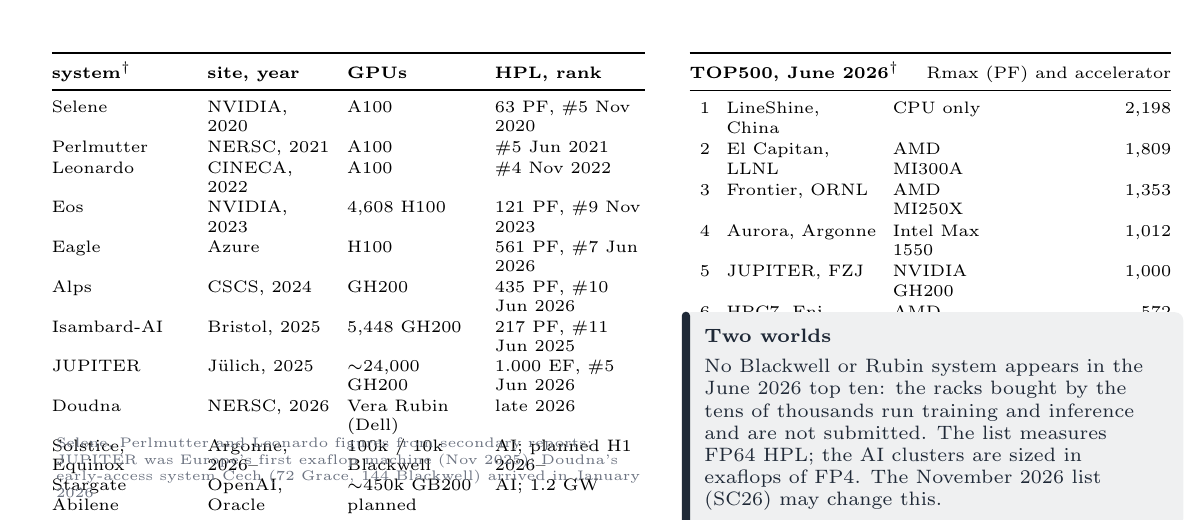
\begin{tikzpicture}
  \useasboundingbox (0,0) rectangle (14.4,5.9);
  \node[anchor=north west,inner sep=0,font=\fontsize{5.8}{6.9}\selectfont] at (0.3,5.6) {%
    \renewcommand{\arraystretch}{1.08}\setlength{\tabcolsep}{2.5pt}%
    \begin{tabular}{@{}>{\raggedright\arraybackslash}p{1.8cm}>{\raggedright\arraybackslash}p{1.6cm}>{\raggedright\arraybackslash}p{1.7cm}>{\raggedright\arraybackslash}p{1.9cm}@{}}
      \toprule
      \textbf{system}$^\dagger$ & \textbf{site, year} & \textbf{GPUs} & \textbf{HPL, rank}\\
      \midrule
      Selene & NVIDIA, 2020 & A100 & 63 PF, \#5 Nov 2020\\
      Perlmutter & NERSC, 2021 & A100 & \#5 Jun 2021\\
      Leonardo & CINECA, 2022 & A100 & \#4 Nov 2022\\
      Eos & NVIDIA, 2023 & 4{,}608 H100 & 121 PF, \#9 Nov 2023\\
      Eagle & Azure & H100 & 561 PF, \#7 Jun 2026\\
      Alps & CSCS, 2024 & GH200 & 435 PF, \#10 Jun 2026\\
      Isambard-AI & Bristol, 2025 & 5{,}448 GH200 & 217 PF, \#11 Jun 2025\\
      JUPITER & J\"ulich, 2025 & ${\sim}$24{,}000 GH200 & 1.000 EF, \#5 Jun 2026\\
      Doudna & NERSC, 2026 & Vera Rubin (Dell) & late 2026\\
      Solstice, Equinox & Argonne, 2026-- & 100k / 10k Blackwell & AI; planned H1 2026--\\
      Stargate Abilene & OpenAI, Oracle & ${\sim}$450k GB200 planned & AI; 1.2 GW\\
      \bottomrule
    \end{tabular}};
  \node[lab,font=\tiny,anchor=north west,text width=7.6cm] at (0.3,0.75) {Selene, Perlmutter and Leonardo figures from secondary reports; JUPITER was Europe's first exaflop machine (Nov 2025); Doudna's early-access system Cech (72 Grace, 144 Blackwell) arrived in January 2026};
  \node[anchor=north west,inner sep=0,font=\fontsize{6.0}{7.1}\selectfont] at (8.4,5.6) {%
    \renewcommand{\arraystretch}{1.08}\setlength{\tabcolsep}{3.0pt}%
    \begin{tabular}{@{}r>{\raggedright\arraybackslash}p{1.9cm}>{\raggedright\arraybackslash}p{1.55cm}r@{}}
      \toprule
      \multicolumn{4}{@{}l@{}}{\textbf{TOP500, June 2026}$^\dagger$ \quad Rmax (PF) and accelerator}\\
      \midrule
      1 & LineShine, China & CPU only & 2{,}198\\
      2 & El Capitan, LLNL & AMD MI300A & 1{,}809\\
      3 & Frontier, ORNL & AMD MI250X & 1{,}353\\
      4 & Aurora, Argonne & Intel Max 1550 & 1{,}012\\
      5 & JUPITER, FZJ & NVIDIA GH200 & 1{,}000\\
      6 & HPC7, Eni & AMD MI300A & 572\\
      7 & Eagle, Azure & NVIDIA H100 & 561\\
      8 & HPC6, Eni & AMD MI250X & 478\\
      9 & Fugaku, RIKEN & CPU only & 442\\
      10 & Alps, CSCS & NVIDIA GH200 & 435\\
      \bottomrule
    \end{tabular}};
  \bgpanels{8.3}{2.3}{5.8cm}{Two worlds}{%
    No Blackwell or Rubin system appears in the June 2026 top ten:
    the racks bought by the tens of thousands run training and
    inference and are not submitted. The list measures FP64 HPL; the
    AI clusters are sized in exaflops of FP4. The November 2026 list
    (SC26) may change this.}
\end{tikzpicture}
\end{frame}

% ---------------------------------------------------------------- 28
\begin{frame}{Scale-up and scale-out: the NVLink domain grew from 8 to 72}
\framesubtitle{Per-GPU link bandwidth rose 19$\times$ since the DGX-1; the number of GPUs on one fabric rose 9$\times$, with 576 on paper.}
\centering
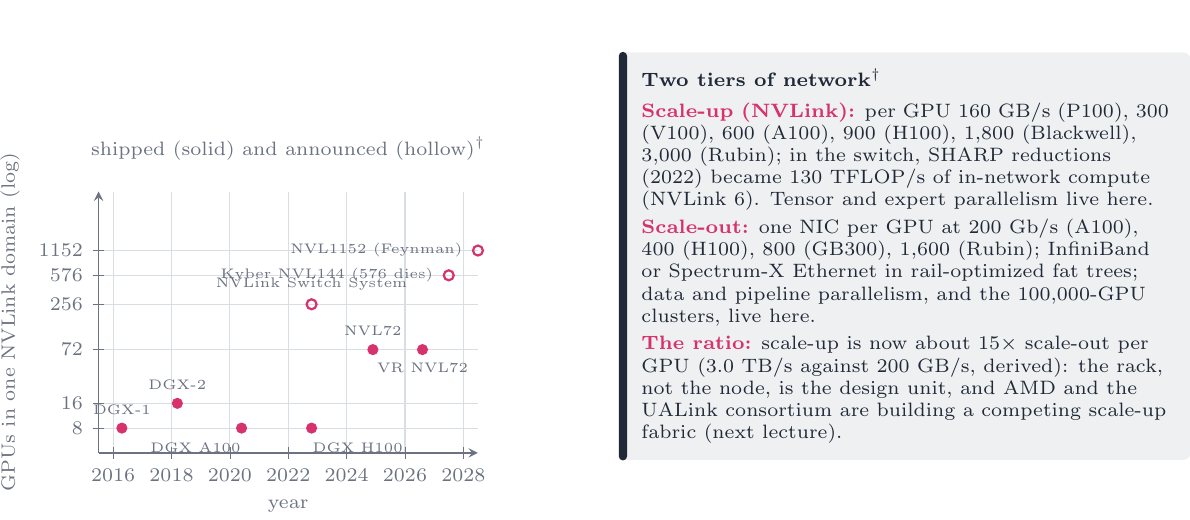
\begin{tikzpicture}
  \useasboundingbox (0,0) rectangle (14.4,5.9);
  \begin{scope}[shift={(0.9,0.5)}]
  \begin{axis}[lecture,width=6.4cm,height=4.9cm,ymode=log,xmin=2015.5,xmax=2028.5,ymin=4,ymax=6000,
      xlabel={year},ylabel={GPUs in one NVLink domain (log)},
      xtick={2016,2018,2020,2022,2024,2026,2028},xticklabel style={/pgf/number format/1000 sep={}},scaled x ticks=false,
      ytick={8,16,72,256,576,1152},yticklabels={8,16,72,256,576,1152},
      title style={font=\scriptsize,text=muted,at={(0.5,1.02)}},title={shipped (solid) and announced (hollow)$^\dagger$}]
    \addplot[outc,only marks,mark=*,mark size=1.8pt] coordinates {(2016.3,8) (2018.2,16) (2020.4,8) (2022.8,8) (2024.9,72) (2026.6,72)};
    \addplot[outc,only marks,mark=o,mark size=1.8pt,line width=0.8pt] coordinates {(2022.8,256) (2027.5,576) (2028.5,1152)};
    \node[font=\tiny,text=muted,anchor=south] at (axis cs:2016.3,9) {DGX-1};
    \node[font=\tiny,text=muted,anchor=south] at (axis cs:2018.2,18) {DGX-2};
    \node[font=\tiny,text=muted,anchor=north east] at (axis cs:2020.7,7) {DGX A100};
    \node[font=\tiny,text=muted,anchor=north west] at (axis cs:2022.5,7) {DGX H100};
    \node[font=\tiny,text=muted,anchor=south] at (axis cs:2022.8,290) {NVLink Switch System};
    \node[font=\tiny,text=muted,anchor=south] at (axis cs:2024.9,82) {NVL72};
    \node[font=\tiny,text=muted,anchor=north] at (axis cs:2026.6,64) {VR NVL72};
    \node[font=\tiny,text=muted,anchor=east] at (axis cs:2027.3,576) {Kyber NVL144 (576 dies)};
    \node[font=\tiny,text=muted,anchor=east] at (axis cs:2028.3,1152) {NVL1152 (Feynman)};
  \end{axis}
  \end{scope}
  \bgpanels{7.5}{5.6}{6.7cm}{Two tiers of network$^\dagger$}{%
    \hl{outc}{Scale-up (NVLink):} per GPU 160 GB/s (P100), 300
    (V100), 600 (A100), 900 (H100), 1{,}800 (Blackwell), 3{,}000
    (Rubin); in the switch, SHARP reductions (2022) became 130
    TFLOP/s of in-network compute (NVLink 6). Tensor and expert
    parallelism live here.\\[2pt]
    \hl{outc}{Scale-out:} one NIC per GPU at 200 Gb/s (A100), 400
    (H100), 800 (GB300), 1{,}600 (Rubin); InfiniBand or Spectrum-X
    Ethernet in rail-optimized fat trees; data and pipeline
    parallelism, and the 100{,}000-GPU clusters, live here.\\[2pt]
    \hl{outc}{The ratio:} scale-up is now about 15$\times$ scale-out
    per GPU (3.0 TB/s against 200 GB/s, derived): the rack, not the
    node, is the design unit, and AMD and the UALink consortium are
    building a competing scale-up fabric (next lecture).}
\end{tikzpicture}
\end{frame}

% ---------------------------------------------------------------- 29
\stage{9}
\begin{frame}{Software: what each generation asked of CUDA}
\framesubtitle{Every hardware feature since Volta arrived with a library that hides it; the programmer's view is a version number.}
\centering
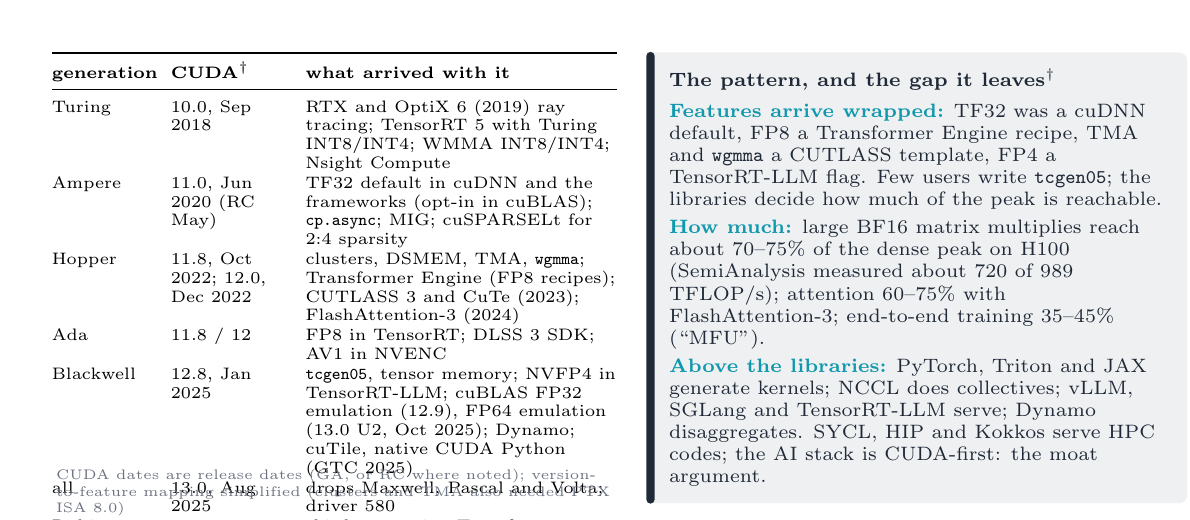
\begin{tikzpicture}
  \useasboundingbox (0,0) rectangle (14.4,5.9);
  \node[anchor=north west,inner sep=0,font=\fontsize{5.7}{6.8}\selectfont] at (0.3,5.6) {%
    \renewcommand{\arraystretch}{1.05}\setlength{\tabcolsep}{3.0pt}%
    \begin{tabular}{@{}>{\raggedright\arraybackslash}p{1.3cm}>{\raggedright\arraybackslash}p{1.5cm}>{\raggedright\arraybackslash}p{3.95cm}@{}}
      \toprule
      \textbf{generation} & \textbf{CUDA}$^\dagger$ & \textbf{what arrived with it}\\
      \midrule
      Turing & 10.0, Sep 2018 & RTX and OptiX 6 (2019) ray tracing; TensorRT 5 with Turing INT8/INT4; WMMA INT8/INT4; Nsight Compute\\
      Ampere & 11.0, Jun 2020 (RC May) & TF32 default in cuDNN and the frameworks (opt-in in cuBLAS); \texttt{cp.async}; MIG; cuSPARSELt for 2:4 sparsity\\
      Hopper & 11.8, Oct 2022; 12.0, Dec 2022 & clusters, DSMEM, TMA, \texttt{wgmma}; Transformer Engine (FP8 recipes); CUTLASS 3 and CuTe (2023); FlashAttention-3 (2024)\\
      Ada & 11.8 / 12 & FP8 in TensorRT; DLSS 3 SDK; AV1 in NVENC\\
      Blackwell & 12.8, Jan 2025 & \texttt{tcgen05}, tensor memory; NVFP4 in TensorRT-LLM; cuBLAS FP32 emulation (12.9), FP64 emulation (13.0 U2, Oct 2025); Dynamo; cuTile, native CUDA Python (GTC 2025)\\
      all & 13.0, Aug 2025 & drops Maxwell, Pascal and Volta; driver 580\\
      Rubin & 13.x, 2026 & third-generation Transformer Engine; NVFP4 training recipes; NVLink 6 collectives\\
      \bottomrule
    \end{tabular}};
  \node[lab,font=\tiny,anchor=north west,text width=7.2cm] at (0.3,0.35) {CUDA dates are release dates (GA, or RC where noted); version-to-feature mapping simplified (clusters and TMA also needed PTX ISA 8.0)};
  \bgpanels{7.85}{5.6}{6.3cm}{The pattern, and the gap it leaves$^\dagger$}{%
    \hl{vc}{Features arrive wrapped:} TF32 was a cuDNN default, FP8 a
    Transformer Engine recipe, TMA and \texttt{wgmma} a CUTLASS
    template, FP4 a TensorRT-LLM flag. Few users write
    \texttt{tcgen05}; the libraries decide how much of the peak is
    reachable.\\[2pt]
    \hl{vc}{How much:} large BF16 matrix multiplies reach about
    70--75\% of the dense peak on H100 (SemiAnalysis measured about
    720 of 989 TFLOP/s); attention 60--75\% with FlashAttention-3;
    end-to-end training 35--45\% (``MFU'').\\[2pt]
    \hl{vc}{Above the libraries:} PyTorch, Triton and JAX generate
    kernels; NCCL does collectives; vLLM, SGLang and TensorRT-LLM
    serve; Dynamo disaggregates. SYCL, HIP and Kokkos serve HPC
    codes; the AI stack is CUDA-first: the moat argument.}
\end{tikzpicture}
\end{frame}

% ---------------------------------------------------------------- 30
\stage{10}
\begin{frame}{The generations in one table}
\framesubtitle{Eight GPUs, 2017--2026: dense peaks, memory, links and power as the datasheets state them.}
\centering
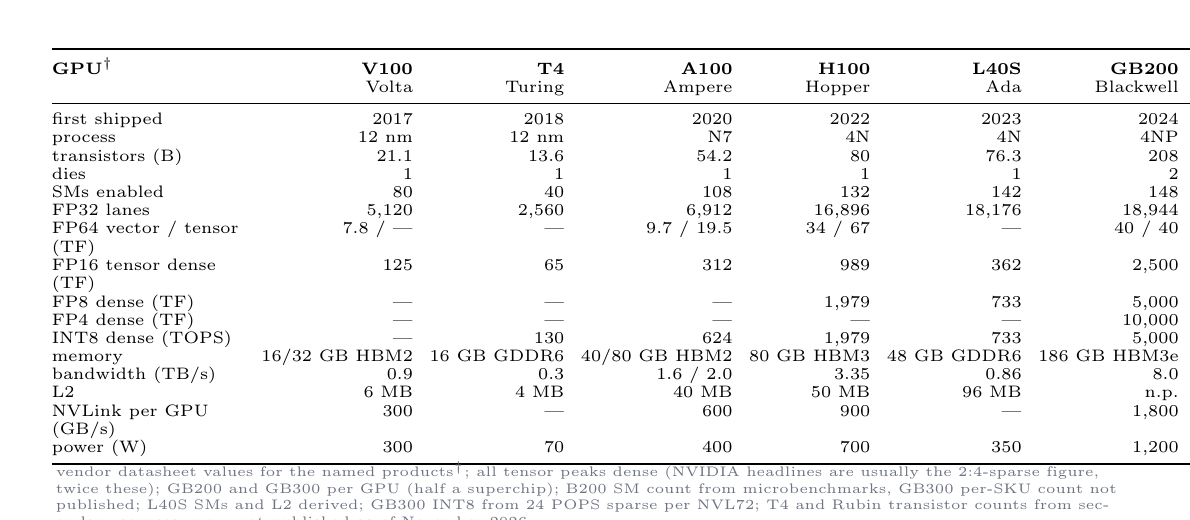
\begin{tikzpicture}
  \useasboundingbox (0,0) rectangle (14.4,5.9);
  \node[anchor=north west,inner sep=0,font=\fontsize{5.7}{6.7}\selectfont] at (0.3,5.65) {%
    \renewcommand{\arraystretch}{0.98}\setlength{\tabcolsep}{3.0pt}%
    \begin{tabular}{@{}>{\raggedright\arraybackslash}p{2.45cm}rrrrrrrr@{}}
      \toprule
      \textbf{GPU}$^\dagger$ & \textbf{V100} & \textbf{T4} & \textbf{A100} & \textbf{H100} & \textbf{L40S} & \textbf{GB200} & \textbf{GB300} & \textbf{Rubin}\\
       & Volta & Turing & Ampere & Hopper & Ada & Blackwell & Bl.\ Ultra & Rubin\\
      \midrule
      first shipped & 2017 & 2018 & 2020 & 2022 & 2023 & 2024 & 2025 & 2026\\
      process & 12 nm & 12 nm & N7 & 4N & 4N & 4NP & 4NP & 3 nm\\
      transistors (B) & 21.1 & 13.6 & 54.2 & 80 & 76.3 & 208 & 208 & 336\\
      dies & 1 & 1 & 1 & 1 & 1 & 2 & 2 & 2\\
      SMs enabled & 80 & 40 & 108 & 132 & 142 & 148 & 160 (full die) & n.p.\\
      FP32 lanes & 5{,}120 & 2{,}560 & 6{,}912 & 16{,}896 & 18{,}176 & 18{,}944 & 20{,}480 & n.p.\\
      FP64 vector / tensor (TF) & 7.8 / --- & --- & 9.7 / 19.5 & 34 / 67 & --- & 40 / 40 & 1.4 & 33 / 33\\
      FP16 tensor dense (TF) & 125 & 65 & 312 & 989 & 362 & 2{,}500 & 2{,}500 & 4{,}000\\
      FP8 dense (TF) & --- & --- & --- & 1{,}979 & 733 & 5{,}000 & 5{,}000 & 17{,}500\\
      FP4 dense (TF) & --- & --- & --- & --- & --- & 10{,}000 & 15{,}000 & 35{,}000\\
      INT8 dense (TOPS) & --- & 130 & 624 & 1{,}979 & 733 & 5{,}000 & about 170 & n.p.\\
      memory & 16/32 GB HBM2 & 16 GB GDDR6 & 40/80 GB HBM2 & 80 GB HBM3 & 48 GB GDDR6 & 186 GB HBM3e & 288 GB HBM3e & 288 GB HBM4\\
      bandwidth (TB/s) & 0.9 & 0.3 & 1.6 / 2.0 & 3.35 & 0.86 & 8.0 & 8.0 & 19.2\\
      L2 & 6 MB & 4 MB & 40 MB & 50 MB & 96 MB & n.p. & n.p. & n.p.\\
      NVLink per GPU (GB/s) & 300 & --- & 600 & 900 & --- & 1{,}800 & 1{,}800 & 3{,}000\\
      power (W) & 300 & 70 & 400 & 700 & 350 & 1{,}200 & 1{,}400 & n.p.\\
      \bottomrule
    \end{tabular}};
  \node[lab,anchor=north west,text width=13.8cm,font=\tiny] at (0.3,0.45) {vendor datasheet values for the named products$^\dagger$; all tensor peaks dense (NVIDIA headlines are usually the 2:4-sparse figure, twice these); GB200 and GB300 per GPU (half a superchip); B200 SM count from microbenchmarks, GB300 per-SKU count not published; L40S SMs and L2 derived; GB300 INT8 from 24 POPS sparse per NVL72; T4 and Rubin transistor counts from secondary sources; n.p.: not published as of November 2026.};
\end{tikzpicture}
\end{frame}

% ---------------------------------------------------------------- 31
\begin{frame}{Summary: what to take from this lecture}
\framesubtitle{The SM template held; the tensor core, formats, memory and links changed; the rack became the GPU.}
\centering
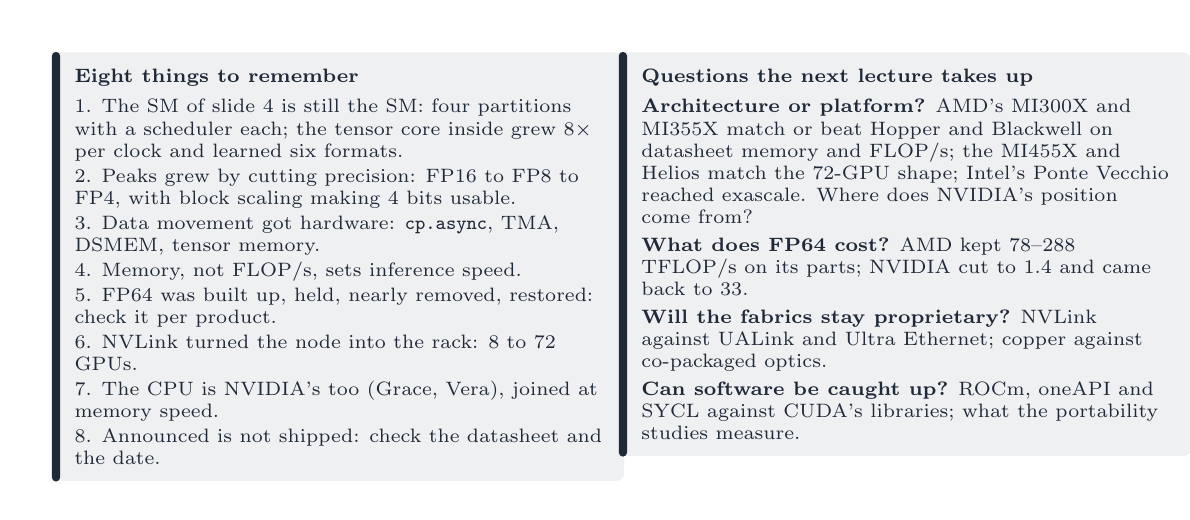
\begin{tikzpicture}
  \useasboundingbox (0,0) rectangle (14.4,5.9);
  \bgpanels{0.3}{5.6}{6.7cm}{Eight things to remember}{%
    1. The SM of slide 4 is still the SM: four partitions with a
    scheduler each; the tensor core inside grew 8$\times$ per clock
    and learned six formats.\\[1pt]
    2. Peaks grew by cutting precision: FP16 to FP8 to FP4, with
    block scaling making 4 bits usable.\\[1pt]
    3. Data movement got hardware: \texttt{cp.async}, TMA, DSMEM,
    tensor memory.\\[1pt]
    4. Memory, not FLOP/s, sets inference speed.\\[1pt]
    5. FP64 was built up, held, nearly removed, restored: check it
    per product.\\[1pt]
    6. NVLink turned the node into the rack: 8 to 72 GPUs.\\[1pt]
    7. The CPU is NVIDIA's too (Grace, Vera), joined at memory speed.\\[1pt]
    8. Announced is not shipped: check the datasheet and the date.}
  \bgpanels{7.5}{5.6}{6.7cm}{Questions the next lecture takes up}{%
    \hl{ink}{Architecture or platform?} AMD's MI300X and MI355X match
    or beat Hopper and Blackwell on datasheet memory and FLOP/s; the
    MI455X and Helios match the 72-GPU shape; Intel's Ponte Vecchio
    reached exascale. Where does NVIDIA's position come from?\\[2pt]
    \hl{ink}{What does FP64 cost?} AMD kept 78--288 TFLOP/s on its
    parts; NVIDIA cut to 1.4 and came back to 33.\\[2pt]
    \hl{ink}{Will the fabrics stay proprietary?} NVLink against UALink
    and Ultra Ethernet; copper against co-packaged optics.\\[2pt]
    \hl{ink}{Can software be caught up?} ROCm, oneAPI and SYCL against
    CUDA's libraries; what the portability studies measure.}
\end{tikzpicture}
\end{frame}

% ---------------------------------------------------------------- 32
\begin{frame}{Sources}
\framesubtitle{Whitepapers and datasheets, papers and talks, systems and reporting; $^\dagger$ marks vendor material.}
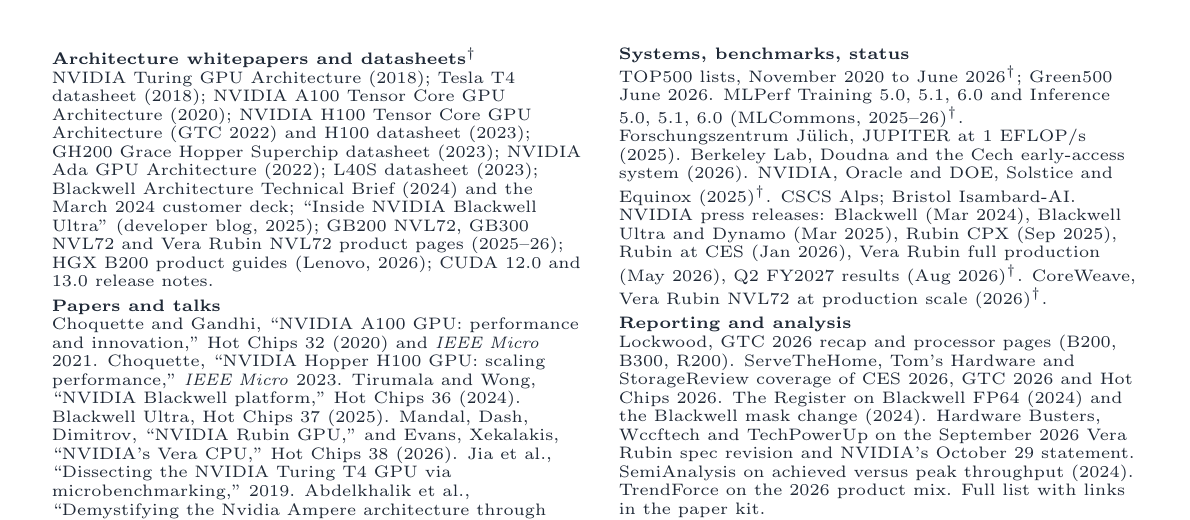
\begin{tikzpicture}
  \useasboundingbox (0,0) rectangle (14.4,5.9);
  \node[anchor=north west,inner sep=0,text width=6.8cm,font=\fontsize{5.6}{6.7}\selectfont,text=ink,align=flush left] at (0.3,5.65) {%
    \textbf{Architecture whitepapers and datasheets}$^\dagger$\\
    NVIDIA Turing GPU Architecture (2018); Tesla T4 datasheet (2018); NVIDIA A100 Tensor Core GPU Architecture (2020); NVIDIA H100 Tensor Core GPU Architecture (GTC 2022) and H100 datasheet (2023); GH200 Grace Hopper Superchip datasheet (2023); NVIDIA Ada GPU Architecture (2022); L40S datasheet (2023); Blackwell Architecture Technical Brief (2024) and the March 2024 customer deck; ``Inside NVIDIA Blackwell Ultra'' (developer blog, 2025); GB200 NVL72, GB300 NVL72 and Vera Rubin NVL72 product pages (2025--26); HGX B200 product guides (Lenovo, 2026); CUDA 12.0 and 13.0 release notes.\\[2pt]
    \textbf{Papers and talks}\\
    Choquette and Gandhi, ``NVIDIA A100 GPU: performance and innovation,'' Hot Chips 32 (2020) and \emph{IEEE Micro} 2021. Choquette, ``NVIDIA Hopper H100 GPU: scaling performance,'' \emph{IEEE Micro} 2023. Tirumala and Wong, ``NVIDIA Blackwell platform,'' Hot Chips 36 (2024). Blackwell Ultra, Hot Chips 37 (2025). Mandal, Dash, Dimitrov, ``NVIDIA Rubin GPU,'' and Evans, Xekalakis, ``NVIDIA's Vera CPU,'' Hot Chips 38 (2026). Jia et al., ``Dissecting the NVIDIA Turing T4 GPU via microbenchmarking,'' 2019. Abdelkhalik et al., ``Demystifying the Nvidia Ampere architecture through microbenchmarking,'' 2022. Luo et al., ``Benchmarking and dissecting the Nvidia Hopper GPU architecture,'' 2024. Jarmusch et al., Blackwell microbenchmarks, 2025 (two papers). Micikevicius et al., ``FP8 formats for deep learning,'' 2022. Rouhani et al., ``Microscaling data formats for deep learning,'' 2023; OCP MX specification 1.0. NVIDIA, ``Introducing NVFP4,'' 2025$^\dagger$; Abecassis et al., ``Pretraining large language models with NVFP4,'' 2025. Shah et al., FlashAttention-3, 2024. NVIDIA Dynamo (2025)$^\dagger$.};
  \node[anchor=north west,inner sep=0,text width=6.6cm,font=\fontsize{5.6}{6.7}\selectfont,text=ink,align=flush left] at (7.5,5.65) {%
    \textbf{Systems, benchmarks, status}\\
    TOP500 lists, November 2020 to June 2026$^\dagger$; Green500 June 2026. MLPerf Training 5.0, 5.1, 6.0 and Inference 5.0, 5.1, 6.0 (MLCommons, 2025--26)$^\dagger$. Forschungszentrum J\"ulich, JUPITER at 1 EFLOP/s (2025). Berkeley Lab, Doudna and the Cech early-access system (2026). NVIDIA, Oracle and DOE, Solstice and Equinox (2025)$^\dagger$. CSCS Alps; Bristol Isambard-AI. NVIDIA press releases: Blackwell (Mar 2024), Blackwell Ultra and Dynamo (Mar 2025), Rubin CPX (Sep 2025), Rubin at CES (Jan 2026), Vera Rubin full production (May 2026), Q2 FY2027 results (Aug 2026)$^\dagger$. CoreWeave, Vera Rubin NVL72 at production scale (2026)$^\dagger$.\\[2pt]
    \textbf{Reporting and analysis}\\
    Lockwood, GTC 2026 recap and processor pages (B200, B300, R200). ServeTheHome, Tom's Hardware and StorageReview coverage of CES 2026, GTC 2026 and Hot Chips 2026. The Register on Blackwell FP64 (2024) and the Blackwell mask change (2024). Hardware Busters, Wccftech and TechPowerUp on the September 2026 Vera Rubin spec revision and NVIDIA's October 29 statement. SemiAnalysis on achieved versus peak throughput (2024). TrendForce on the 2026 product mix. Full list with links in the paper kit.};
\end{tikzpicture}
\end{frame}
\end{document}
